\section{Results}
\label{sec:results}
In this section we present the results of the experiments defined in section \ref{sec:experiments}. The results will be grouped per scenario. We start by a short summary of each scenario, followed by presenting the overall damage of the system in each of the scenarios, as it is the key indicator of the performance of the system. We then present the other metrics that we defined in section \ref{ssec:metrics}.

\subsection{Scenario 1: No Changes}
\textit{In this scenario, no external changes are made to the infrastructure. The purpose of this scenario is to see how the system behaves when no changes are made.}

To introduce the graphs and what they mean, this subsection will go through the graphs in a bit more detail than in the subsections afterwards. 

\begin{figure}[H]
    \centering
    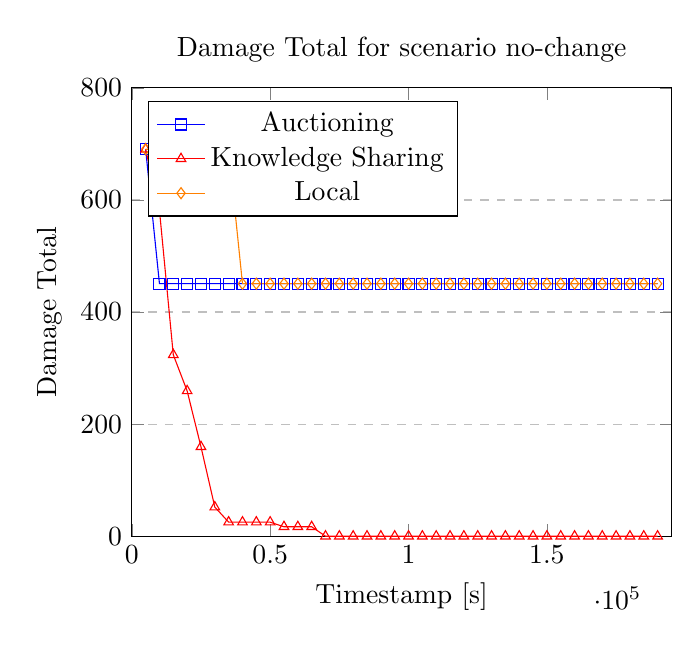
\begin{tikzpicture}
\begin{axis}[
    title={Damage Total for scenario no-change},
    xlabel={Timestamp [s]},
    ylabel={Damage Total},
    xmin=0, xmax=195000,
    ymin=0, ymax=800,
    legend pos=north west,
    ymajorgrids=true,
    grid style=dashed,
]

\addplot[
    color=blue,
    mark=square,
    ]
    coordinates {
    (5000,690.52)(10000,450.57)(15000,450.57)(20000,450.57)(25000,450.57)(30000,450.57)(35000,450.57)(40000,450.57)(45000,450.57)(50000,450.57)(55000,450.57)(60000,450.57)(65000,450.57)(70000,450.57)(75000,450.57)(80000,450.57)(85000,450.57)(90000,450.57)(95000,450.57)(100000,450.57)(105000,450.57)(110000,450.57)(115000,450.57)(120000,450.57)(125000,450.57)(130000,450.57)(135000,450.57)(140000,450.57)(145000,450.57)(150000,450.57)(155000,450.57)(160000,450.57)(165000,450.57)(170000,450.57)(175000,450.57)(180000,450.57)(185000,450.57)(190000,450.57)
    };
    \addlegendentry{Auctioning}
\addplot[
    color=red,
    mark=triangle,
    ]
    coordinates {
    (5000,690.52)(10000,581.45)(15000,323.71)(20000,259.27)(25000,159.58)(30000,51.98)(35000,25.08)(40000,25.08)(45000,25.08)(50000,25.08)(55000,16.82)(60000,16.82)(65000,16.82)(70000,0.00)(75000,0.00)(80000,0.00)(85000,0.00)(90000,0.00)(95000,0.00)(100000,0.00)(105000,0.00)(110000,0.00)(115000,0.00)(120000,0.00)(125000,0.00)(130000,0.00)(135000,0.00)(140000,0.00)(145000,0.00)(150000,0.00)(155000,0.00)(160000,0.00)(165000,0.00)(170000,0.00)(175000,0.00)(180000,0.00)(185000,0.00)(190000,0.00)
    };
    \addlegendentry{Knowledge Sharing}
\addplot[
    color=orange,
    mark=diamond,
    ]
    coordinates {
    (5000,690.52)(10000,690.52)(15000,690.52)(20000,690.52)(25000,690.52)(30000,690.52)(35000,690.52)(40000,450.57)(45000,450.57)(50000,450.57)(55000,450.57)(60000,450.57)(65000,450.57)(70000,450.57)(75000,450.57)(80000,450.57)(85000,450.57)(90000,450.57)(95000,450.57)(100000,450.57)(105000,450.57)(110000,450.57)(115000,450.57)(120000,450.57)(125000,450.57)(130000,450.57)(135000,450.57)(140000,450.57)(145000,450.57)(150000,450.57)(155000,450.57)(160000,450.57)(165000,450.57)(170000,450.57)(175000,450.57)(180000,450.57)(185000,450.57)(190000,450.57)
    };
    \addlegendentry{Local}
    
\end{axis}
\end{tikzpicture}
    \caption{This graph shows the overall damage of the system in the scenario where no changes are made overtime.}
    \label{fig:overall-damage-no-change}
\end{figure}

From figure \ref{fig:overall-damage-no-change} we see that the agent with the Local-feature set (from here-on \textit{local-agent}) slowly reduces the overall damage of the network, but is unable to get any lower than around $275$, and stays at this value after roughly the first $50$ seconds.
Within the first $25$ seconds, the knowledge-sharing agents are able to reduce the overall damage to around $220$, but is unable to get any lower than this. 
Finally, the auctioning are able to reduce the damage to roughly $80$, but is only able to get there after $80$ seconds.
The lowest value is for the auctioning agent at $35\%$ of the damage the local-agent.

\begin{figure}[H]
    \centering
    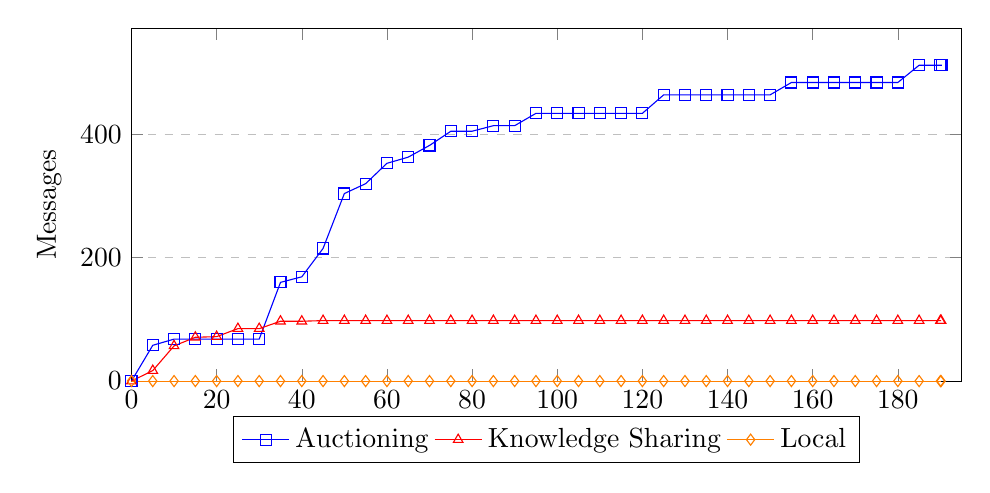
\begin{tikzpicture}
\begin{axis}[
    xlabel={Timestamp [s]},
    ylabel={Messages},
    xmin=0, xmax=195000,
    ymin=0, ymax=572,
    legend columns=-1,
    legend style={at={(0.5,-0.1)},anchor=north},
    ymajorgrids=true,
    grid style=dashed,
    width=\textwidth,
    height=0.5\textwidth,
    scaled x ticks=base 10:-3,
    xtick scale label code/.code={}
]

	\addplot[color=blue,mark=square] coordinates {
        (0,0)(5000,58)(10000,68)(15000,68)(20000,68)(25000,68)(30000,68)(35000,160)(40000,169)(45000,215)(50000,304)(55000,320)(60000,353)(65000,363)(70000,382)(75000,405)(80000,405)(85000,414)(90000,414)(95000,434)(100000,434)(105000,434)(110000,434)(115000,434)(120000,434)(125000,464)(130000,464)(135000,464)(140000,464)(145000,464)(150000,464)(155000,484)(160000,484)(165000,484)(170000,484)(175000,484)(180000,484)(185000,512)(190000,512)(190364,512)
    };
    \addlegendentry{Auctioning}
	\addplot[color=red,mark=triangle] coordinates {
        (0,0)(5000,17)(10000,57)(15000,71)(20000,72)(25000,85)(30000,85)(35000,97)(40000,97)(45000,98)(50000,98)(55000,98)(60000,98)(65000,98)(70000,98)(75000,98)(80000,98)(85000,98)(90000,98)(95000,98)(100000,98)(105000,98)(110000,98)(115000,98)(120000,98)(125000,98)(130000,98)(135000,98)(140000,98)(145000,98)(150000,98)(155000,98)(160000,98)(165000,98)(170000,98)(175000,98)(180000,98)(185000,98)(190000,98)(190165,98)
    };
    \addlegendentry{Knowledge Sharing}
	\addplot[color=orange,mark=diamond] coordinates {
        (0,0)(5000,0)(10000,0)(15000,0)(20000,0)(25000,0)(30000,0)(35000,0)(40000,0)(45000,0)(50000,0)(55000,0)(60000,0)(65000,0)(70000,0)(75000,0)(80000,0)(85000,0)(90000,0)(95000,0)(100000,0)(105000,0)(110000,0)(115000,0)(120000,0)(125000,0)(130000,0)(135000,0)(140000,0)(145000,0)(150000,0)(155000,0)(160000,0)(165000,0)(170000,0)(175000,0)(180000,0)(185000,0)(190000,0)(190150,0)
    };
    \addlegendentry{Local}




\end{axis}
\end{tikzpicture}
    \caption{Graph showing the total amount of messages sent between agents in the scenario where no changes are made overtime.}
    \label{fig:messages-no-change}
\end{figure}

In figure \ref{fig:messages-no-change} we can see that the local-agent shares no messages, as this feature-set does not allow for it. The auctioning agent sends the most messages. After $80$ seconds all agents have found a stable point damage-wise, and this is also visible from the messages for the auctioning agents. At this point the auctioning agents have sent almost three times as much as the knowledge-sharing agents. This can be explained by the fact that the auctioning agents have a total of $11$ events that can be sent to other agents, compared to the knowledge-sharing agent, which has only $4$ types of messages. This $4 / 11$ ratio is roughly the same as the ratio between the amount of messages sent by the auctioning and knowledge-sharing agents. However, this could be a coincidence, and more research would be needed for this assumption. During an auction participating nodes send on average $4$ messages per participating node, which could also explain the difference in messages sent. 

The message count for auctioning nodes goes up roughly every $30$ second, which is the interval at which any agent will start identifying risks if it has received no messages. During this time the agents share some knowledge, sometimes try an auction but then stop because there are no proposals to be made.

\begin{figure}[H]
    \centering
    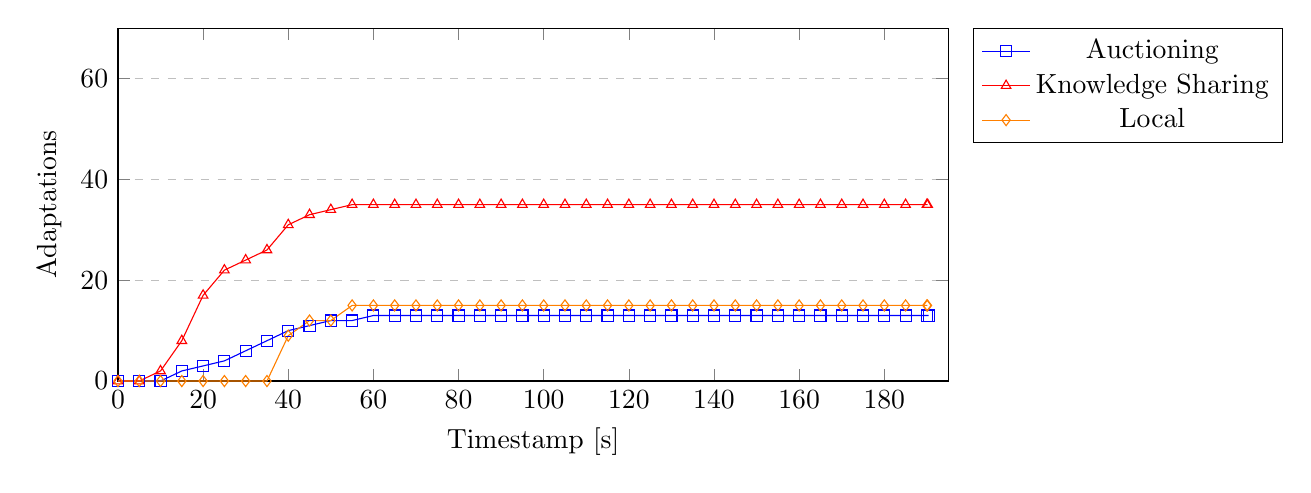
\begin{tikzpicture}
\begin{axis}[
    xlabel={Timestamp [s]},
    ylabel={Adaptations},
    xmin=0, xmax=195000,
    ymin=0, ymax=70,
    legend pos=outer north east,
    ymajorgrids=true,
    grid style=dashed,
    width=\textwidth,
    height=0.5\textwidth,
    scaled x ticks=base 10:-3,
    xtick scale label code/.code={}
]

	\addplot[color=blue,mark=square] coordinates {
        (0,0)(5000,0)(10000,0)(15000,2)(20000,3)(25000,4)(30000,6)(35000,8)(40000,10)(45000,11)(50000,12)(55000,12)(60000,13)(65000,13)(70000,13)(75000,13)(80000,13)(85000,13)(90000,13)(95000,13)(100000,13)(105000,13)(110000,13)(115000,13)(120000,13)(125000,13)(130000,13)(135000,13)(140000,13)(145000,13)(150000,13)(155000,13)(160000,13)(165000,13)(170000,13)(175000,13)(180000,13)(185000,13)(190000,13)(190434,13)
    };
    \addlegendentry{Auctioning}
	\addplot[color=red,mark=triangle] coordinates {
        (0,0)(5000,0)(10000,2)(15000,8)(20000,17)(25000,22)(30000,24)(35000,26)(40000,31)(45000,33)(50000,34)(55000,35)(60000,35)(65000,35)(70000,35)(75000,35)(80000,35)(85000,35)(90000,35)(95000,35)(100000,35)(105000,35)(110000,35)(115000,35)(120000,35)(125000,35)(130000,35)(135000,35)(140000,35)(145000,35)(150000,35)(155000,35)(160000,35)(165000,35)(170000,35)(175000,35)(180000,35)(185000,35)(190000,35)(190190,35)
    };
    \addlegendentry{Knowledge Sharing}
	\addplot[color=orange,mark=diamond] coordinates {
        (0,0)(5000,0)(10000,0)(15000,0)(20000,0)(25000,0)(30000,0)(35000,0)(40000,9)(45000,12)(50000,12)(55000,15)(60000,15)(65000,15)(70000,15)(75000,15)(80000,15)(85000,15)(90000,15)(95000,15)(100000,15)(105000,15)(110000,15)(115000,15)(120000,15)(125000,15)(130000,15)(135000,15)(140000,15)(145000,15)(150000,15)(155000,15)(160000,15)(165000,15)(170000,15)(175000,15)(180000,15)(185000,15)(190000,15)(190138,15)
    };
    \addlegendentry{Local}




\end{axis}
\end{tikzpicture}
    \caption{Graph showing the total amount of adaptations applied by agents in the scenario where no changes are made overtime.}
    \label{fig:proposals-no-change}
\end{figure}

From figure \ref{fig:proposals-no-change} we can see that the knowledge-sharing agent applies the most adaptations, followed by the auctioning agent. The local-agent applies the least adaptations. The knowledge-sharing agent applies almost $3$ times  more adaptations than the local agent. The knowledge-sharing agent has a steep increase in the first $25$ seconds, after which it becomes more stable. The auctioning agent has a slower increase, but is applying adaptations at a steady rate. This is to be expected as any adaptation will be negotiated first, which takes time.

\begin{figure}[H]
    \centering
        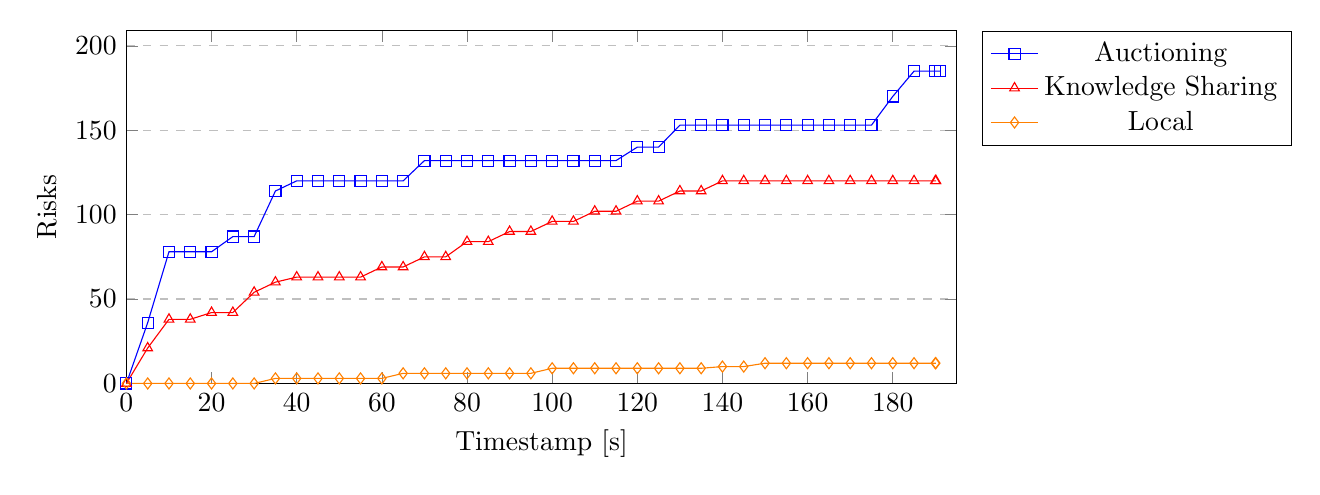
\begin{tikzpicture}
\begin{axis}[
    xlabel={Timestamp [s]},
    ylabel={Risks},
    xmin=0, xmax=195000,
    ymin=0, ymax=209,
    legend pos=outer north east,
    ymajorgrids=true,
    grid style=dashed,
    width=\textwidth,
    height=0.5\textwidth,
    scaled x ticks=base 10:-3,
    xtick scale label code/.code={}
]

	\addplot[color=blue,mark=square] coordinates {
        (0,0)(5000,36)(10000,78)(15000,78)(20000,78)(25000,87)(30000,87)(35000,114)(40000,120)(45000,120)(50000,120)(55000,120)(60000,120)(65000,120)(70000,132)(75000,132)(80000,132)(85000,132)(90000,132)(95000,132)(100000,132)(105000,132)(110000,132)(115000,132)(120000,140)(125000,140)(130000,153)(135000,153)(140000,153)(145000,153)(150000,153)(155000,153)(160000,153)(165000,153)(170000,153)(175000,153)(180000,170)(185000,185)(190000,185)(191066,185)
    };
    \addlegendentry{Auctioning}
	\addplot[color=red,mark=triangle] coordinates {
        (0,0)(5000,21)(10000,38)(15000,38)(20000,42)(25000,42)(30000,54)(35000,60)(40000,63)(45000,63)(50000,63)(55000,63)(60000,69)(65000,69)(70000,75)(75000,75)(80000,84)(85000,84)(90000,90)(95000,90)(100000,96)(105000,96)(110000,102)(115000,102)(120000,108)(125000,108)(130000,114)(135000,114)(140000,120)(145000,120)(150000,120)(155000,120)(160000,120)(165000,120)(170000,120)(175000,120)(180000,120)(185000,120)(190000,120)(190155,120)
    };
    \addlegendentry{Knowledge Sharing}
	\addplot[color=orange,mark=diamond] coordinates {
        (0,0)(5000,0)(10000,0)(15000,0)(20000,0)(25000,0)(30000,0)(35000,3)(40000,3)(45000,3)(50000,3)(55000,3)(60000,3)(65000,6)(70000,6)(75000,6)(80000,6)(85000,6)(90000,6)(95000,6)(100000,9)(105000,9)(110000,9)(115000,9)(120000,9)(125000,9)(130000,9)(135000,9)(140000,10)(145000,10)(150000,12)(155000,12)(160000,12)(165000,12)(170000,12)(175000,12)(180000,12)(185000,12)(190000,12)(190110,12)
    };
    \addlegendentry{Local}




\end{axis}
\end{tikzpicture}
    \caption{Graph showing the number of unique risks detected by agents in the scenario where no changes are made overtime.}
    \label{fig:risk-count-no-change}
\end{figure}

Figure \ref{fig:risk-count-no-change} shows that the knowledge-sharing agent detects the most risks, followed by the auctioning agent with roughly $70\%$ of the risks found. The local-agent detects the least amount of risks at only $10\%$ compared to the auctioning agent. It is to be expected that the local-agents can only detect a fraction of what the other agents detect, as the risks that can be deduced from only their local knowledge is limited.

\begin{figure}[H]
    \centering
        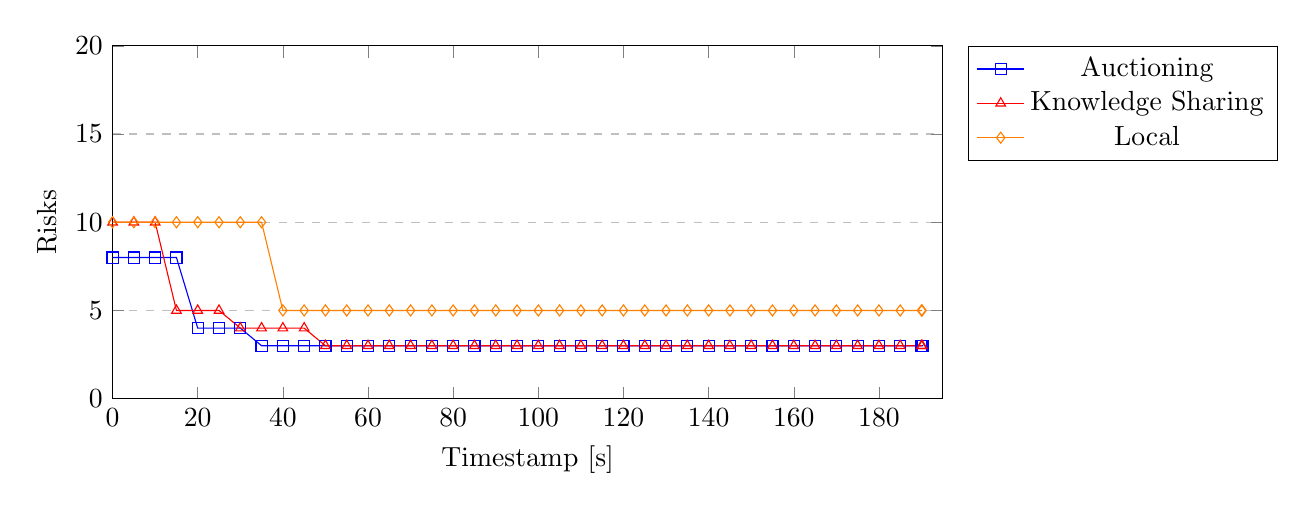
\begin{tikzpicture}
\begin{axis}[
    xlabel={Timestamp [s]},
    ylabel={Risks},
    xmin=0, xmax=195000,
    ymin=0, ymax=20,
    legend pos=outer north east,
    ymajorgrids=true,
    grid style=dashed,
    width=\textwidth,
    height=0.5\textwidth,
    scaled x ticks=base 10:-3,
    xtick scale label code/.code={}
]

	\addplot[color=blue,mark=square] coordinates {
        (0,8)(5000,8)(10000,8)(15000,8)(20000,4)(25000,4)(30000,4)(35000,3)(40000,3)(45000,3)(50000,3)(55000,3)(60000,3)(65000,3)(70000,3)(75000,3)(80000,3)(85000,3)(90000,3)(95000,3)(100000,3)(105000,3)(110000,3)(115000,3)(120000,3)(125000,3)(130000,3)(135000,3)(140000,3)(145000,3)(150000,3)(155000,3)(160000,3)(165000,3)(170000,3)(175000,3)(180000,3)(185000,3)(190000,3)(190439,3)
    };
    \addlegendentry{Auctioning}
	\addplot[color=red,mark=triangle] coordinates {
        (0,10)(5000,10)(10000,10)(15000,5)(20000,5)(25000,5)(30000,4)(35000,4)(40000,4)(45000,4)(50000,3)(55000,3)(60000,3)(65000,3)(70000,3)(75000,3)(80000,3)(85000,3)(90000,3)(95000,3)(100000,3)(105000,3)(110000,3)(115000,3)(120000,3)(125000,3)(130000,3)(135000,3)(140000,3)(145000,3)(150000,3)(155000,3)(160000,3)(165000,3)(170000,3)(175000,3)(180000,3)(185000,3)(190000,3)(190147,3)
    };
    \addlegendentry{Knowledge Sharing}
	\addplot[color=orange,mark=diamond] coordinates {
        (0,10)(5000,10)(10000,10)(15000,10)(20000,10)(25000,10)(30000,10)(35000,10)(40000,5)(45000,5)(50000,5)(55000,5)(60000,5)(65000,5)(70000,5)(75000,5)(80000,5)(85000,5)(90000,5)(95000,5)(100000,5)(105000,5)(110000,5)(115000,5)(120000,5)(125000,5)(130000,5)(135000,5)(140000,5)(145000,5)(150000,5)(155000,5)(160000,5)(165000,5)(170000,5)(175000,5)(180000,5)(185000,5)(190000,5)(190136,5)
    };
    \addlegendentry{Local}




\end{axis}
\end{tikzpicture}
    \caption{Graph showing the number of remaining risks in the infrastructure in the scenario where no changes are made overtime.}
    \label{fig:risk-remaining-no-change}
\end{figure}

When comparing figure \ref{fig:overall-damage-no-change} to figure \ref{fig:risk-remaining-no-change}, we see that the graphs are following the same trend. This is to be expected, as the overall damage is calculated by summing the damage of all the remaining risks.

\begin{figure}[H]
    \centering
        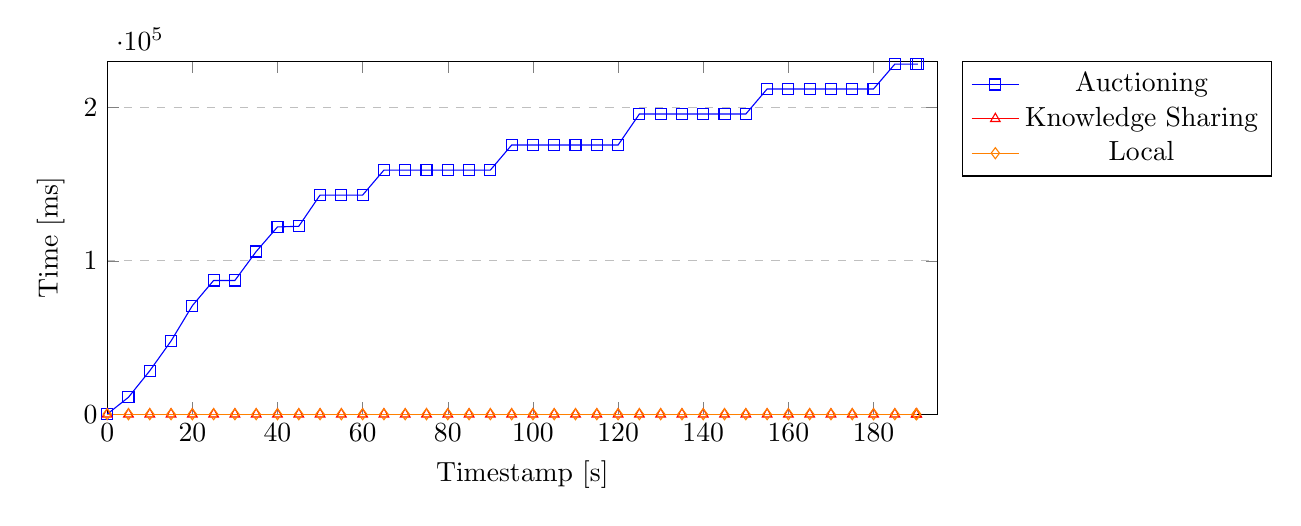
\begin{tikzpicture}
\begin{axis}[
    xlabel={Timestamp [s]},
    ylabel={Time [ms]},
    xmin=0, xmax=195000,
    ymin=0, ymax=230023,
    legend pos=outer north east,
    ymajorgrids=true,
    grid style=dashed,
    width=\textwidth,
    height=0.5\textwidth,
    scaled x ticks=base 10:-3,
    xtick scale label code/.code={}
]

	\addplot[color=blue,mark=square] coordinates {
        (0,0)(5000,11025)(10000,28282)(15000,47709)(20000,70713)(25000,87182)(30000,87182)(35000,106048)(40000,122066)(45000,122489)(50000,142841)(55000,142841)(60000,142841)(65000,159124)(70000,159124)(75000,159124)(80000,159124)(85000,159124)(90000,159124)(95000,175471)(100000,175471)(105000,175471)(110000,175471)(115000,175471)(120000,175471)(125000,195658)(130000,195658)(135000,195658)(140000,195658)(145000,195658)(150000,195658)(155000,212013)(160000,212013)(165000,212013)(170000,212013)(175000,212013)(180000,212013)(185000,228231)(190000,228231)(190439,228231)
    };
    \addlegendentry{Auctioning}
	\addplot[color=red,mark=triangle] coordinates {
        (0,0)(5000,0)(10000,0)(15000,0)(20000,0)(25000,0)(30000,0)(35000,0)(40000,0)(45000,0)(50000,0)(55000,0)(60000,0)(65000,0)(70000,0)(75000,0)(80000,0)(85000,0)(90000,0)(95000,0)(100000,0)(105000,0)(110000,0)(115000,0)(120000,0)(125000,0)(130000,0)(135000,0)(140000,0)(145000,0)(150000,0)(155000,0)(160000,0)(165000,0)(170000,0)(175000,0)(180000,0)(185000,0)(190000,0)(190147,0)
    };
    \addlegendentry{Knowledge Sharing}
	\addplot[color=orange,mark=diamond] coordinates {
        (0,0)(5000,0)(10000,0)(15000,0)(20000,0)(25000,0)(30000,0)(35000,0)(40000,0)(45000,0)(50000,0)(55000,0)(60000,0)(65000,0)(70000,0)(75000,0)(80000,0)(85000,0)(90000,0)(95000,0)(100000,0)(105000,0)(110000,0)(115000,0)(120000,0)(125000,0)(130000,0)(135000,0)(140000,0)(145000,0)(150000,0)(155000,0)(160000,0)(165000,0)(170000,0)(175000,0)(180000,0)(185000,0)(190000,0)(190136,0)
    };
    \addlegendentry{Local}




\end{axis}
\end{tikzpicture}
    \caption{Graph showing the sum of time spent auctioning by agents in the scenario where no changes are made overtime.}
    \label{fig:auctioning-time-no-change}
\end{figure}

Figure \ref{fig:auctioning-time-no-change} shows that the auctioning agents is the only agent that spends time auctioning. This is to be expected, as the auctioning agents are the only agents that can auction.

\begin{figure}[H]
    \centering
        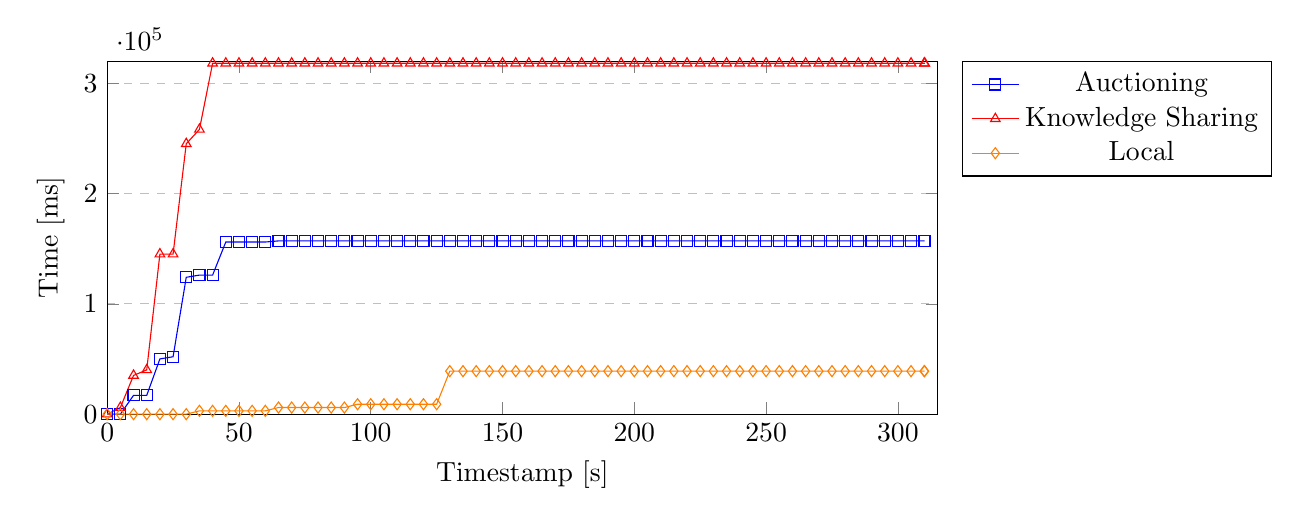
\begin{tikzpicture}
\begin{axis}[
    xlabel={Timestamp [s]},
    ylabel={Time [ms]},
    xmin=0, xmax=315000,
    ymin=0, ymax=320032,
    legend pos=outer north east,
    ymajorgrids=true,
    grid style=dashed,
    width=\textwidth,
    height=0.5\textwidth,
    scaled x ticks=base 10:-3,
    xtick scale label code/.code={}
]

	\addplot[color=blue,mark=square] coordinates {
        (0,0)(5000,0)(10000,17072)(15000,17072)(20000,50094)(25000,52106)(30000,124138)(35000,126144)(40000,126144)(45000,156154)(50000,156154)(55000,156154)(60000,156154)(65000,157158)(70000,157158)(75000,157158)(80000,157158)(85000,157158)(90000,157158)(95000,157158)(100000,157158)(105000,157158)(110000,157158)(115000,157158)(120000,157158)(125000,157158)(130000,157158)(135000,157158)(140000,157158)(145000,157158)(150000,157158)(155000,157158)(160000,157158)(165000,157158)(170000,157158)(175000,157158)(180000,157158)(185000,157158)(190000,157158)(195000,157158)(200000,157158)(205000,157158)(210000,157158)(215000,157158)(220000,157158)(225000,157158)(230000,157158)(235000,157158)(240000,157158)(245000,157158)(250000,157158)(255000,157158)(260000,157158)(265000,157158)(270000,157158)(275000,157158)(280000,157158)(285000,157158)(290000,157158)(295000,157158)(300000,157158)(305000,157158)(310000,157158)(310159,157158)
    };
    \addlegendentry{Auctioning}
	\addplot[color=red,mark=triangle] coordinates {
        (0,0)(5000,6039)(10000,35135)(15000,40149)(20000,145217)(25000,145217)(30000,245261)(35000,258272)(40000,318293)(45000,318293)(50000,318293)(55000,318293)(60000,318293)(65000,318293)(70000,318293)(75000,318293)(80000,318293)(85000,318293)(90000,318293)(95000,318293)(100000,318293)(105000,318293)(110000,318293)(115000,318293)(120000,318293)(125000,318293)(130000,318293)(135000,318293)(140000,318293)(145000,318293)(150000,318293)(155000,318293)(160000,318293)(165000,318293)(170000,318293)(175000,318293)(180000,318293)(185000,318293)(190000,318293)(195000,318293)(200000,318293)(205000,318293)(210000,318293)(215000,318293)(220000,318293)(225000,318293)(230000,318293)(235000,318293)(240000,318293)(245000,318293)(250000,318293)(255000,318293)(260000,318293)(265000,318293)(270000,318293)(275000,318293)(280000,318293)(285000,318293)(290000,318293)(295000,318293)(300000,318293)(305000,318293)(310000,318293)(310212,318293)
    };
    \addlegendentry{Knowledge Sharing}
	\addplot[color=orange,mark=diamond] coordinates {
        (0,0)(5000,0)(10000,0)(15000,0)(20000,0)(25000,0)(30000,0)(35000,3012)(40000,3012)(45000,3012)(50000,3012)(55000,3012)(60000,3012)(65000,6020)(70000,6020)(75000,6020)(80000,6020)(85000,6020)(90000,6020)(95000,9026)(100000,9026)(105000,9026)(110000,9026)(115000,9026)(120000,9026)(125000,9026)(130000,39035)(135000,39035)(140000,39035)(145000,39035)(150000,39035)(155000,39035)(160000,39035)(165000,39035)(170000,39035)(175000,39035)(180000,39035)(185000,39035)(190000,39035)(195000,39035)(200000,39035)(205000,39035)(210000,39035)(215000,39035)(220000,39035)(225000,39035)(230000,39035)(235000,39035)(240000,39035)(245000,39035)(250000,39035)(255000,39035)(260000,39035)(265000,39035)(270000,39035)(275000,39035)(280000,39035)(285000,39035)(290000,39035)(295000,39035)(300000,39035)(305000,39035)(310000,39035)(310137,39035)
    };
    \addlegendentry{Local}




\end{axis}
\end{tikzpicture}
    \caption{Graph showing the sum of time spent adapting by agents in the scenario where no changes are made overtime.}
    \label{fig:adapting-time-no-change}
\end{figure}

Figure \ref{fig:adapting-time-no-change} shows that the knowledge-sharing agents spends the most amount of time adapting during this scenario. The auctioning agent is second, and the local agent spends the least amount of time adapting. This is inline with the amount of adaptations applied.

\subsection{Scenario 2: Risk Introduction}
\label{ssec:scenario-2-results}
\textit{This scenario introduces a risk to the infrastructure after $180$ seconds. The purpose of this scenario is to see how the system behaves when a new risk is introduced.}

\begin{figure}[H]
    \centering
    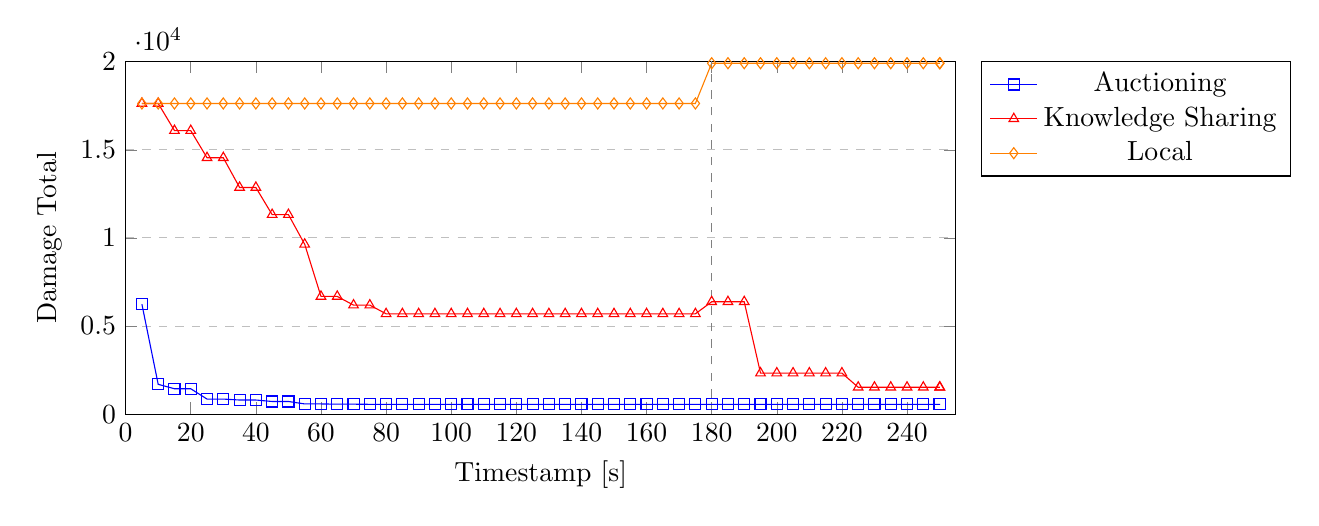
\begin{tikzpicture}
\begin{axis}[
    xlabel={Timestamp [s]},
    ylabel={Damage Total},
    xmin=0, xmax=255000,
    ymin=0, ymax=20020,
    legend pos=outer north east,
    ymajorgrids=true,
    grid style=dashed,
    width=\textwidth,
    height=0.5\textwidth,
    scaled x ticks=base 10:-3,
    xtick scale label code/.code={}
]

	\addplot[color=blue,mark=square] coordinates {
        (5000,6236.51)(10000,1693.70)(15000,1442.78)(20000,1442.78)(25000,857.00)(30000,857.00)(35000,803.10)(40000,803.10)(45000,720.33)(50000,720.33)(55000,580.88)(60000,580.88)(65000,567.64)(70000,567.64)(75000,559.15)(80000,556.95)(85000,556.95)(90000,556.95)(95000,556.95)(100000,556.95)(105000,556.95)(110000,556.95)(115000,556.95)(120000,556.95)(125000,556.95)(130000,556.95)(135000,556.95)(140000,556.95)(145000,556.95)(150000,556.95)(155000,556.95)(160000,556.95)(165000,556.95)(170000,556.95)(175000,556.95)(180000,556.95)(185000,560.22)(190000,560.22)(195000,560.22)(200000,560.22)(205000,560.22)(210000,560.22)(215000,560.22)(220000,560.22)(225000,560.22)(230000,560.22)(235000,560.22)(240000,560.22)(245000,560.22)(250000,560.22)(250139,560.22)
    };
    \addlegendentry{Auctioning}
	\addplot[color=red,mark=triangle] coordinates {
        (5000,17629.95)(10000,17629.95)(15000,16089.24)(20000,16089.24)(25000,14548.54)(30000,14548.54)(35000,12864.04)(40000,12864.04)(45000,11323.33)(50000,11323.33)(55000,9638.83)(60000,6680.68)(65000,6680.68)(70000,6187.65)(75000,6187.65)(80000,5694.63)(85000,5694.63)(90000,5694.63)(95000,5694.63)(100000,5694.63)(105000,5694.63)(110000,5694.63)(115000,5694.63)(120000,5694.63)(125000,5694.63)(130000,5694.63)(135000,5694.63)(140000,5694.63)(145000,5694.63)(150000,5694.63)(155000,5694.63)(160000,5694.63)(165000,5694.63)(170000,5694.63)(175000,5694.63)(180000,6377.52)(185000,6377.52)(190000,6377.52)(195000,2331.23)(200000,2331.23)(205000,2331.23)(210000,2331.23)(215000,2331.23)(220000,2331.23)(225000,1526.78)(230000,1526.78)(235000,1526.78)(240000,1526.78)(245000,1526.78)(250000,1526.78)(250111,1526.78)
    };
    \addlegendentry{Knowledge Sharing}
	\addplot[color=orange,mark=diamond] coordinates {
        (5000,17629.95)(10000,17629.95)(15000,17629.95)(20000,17629.95)(25000,17629.95)(30000,17629.95)(35000,17629.95)(40000,17629.95)(45000,17629.95)(50000,17629.95)(55000,17629.95)(60000,17629.95)(65000,17629.95)(70000,17629.95)(75000,17629.95)(80000,17629.95)(85000,17629.95)(90000,17629.95)(95000,17629.95)(100000,17629.95)(105000,17629.95)(110000,17629.95)(115000,17629.95)(120000,17629.95)(125000,17629.95)(130000,17629.95)(135000,17629.95)(140000,17629.95)(145000,17629.95)(150000,17629.95)(155000,17629.95)(160000,17629.95)(165000,17629.95)(170000,17629.95)(175000,17629.95)(180000,19913.02)(185000,19913.02)(190000,19913.02)(195000,19913.02)(200000,19913.02)(205000,19913.02)(210000,19913.02)(215000,19913.02)(220000,19913.02)(225000,19913.02)(230000,19913.02)(235000,19913.02)(240000,19913.02)(245000,19913.02)(250000,19913.02)(250115,19913.02)
    };
    \addlegendentry{Local}

	\addplot[color=gray, dashed,] coordinates {(180000,0) (180000,20020)};


\end{axis}
\end{tikzpicture}
    \caption{This graph shows the overall damage of the system in the risk introduction scenario. The damage is shown for each of the three strategies. The vertical lines indicate the time at which a risk is introduced.}
    \label{fig:overall-damage-inroduce-risk}
\end{figure}

Figure \ref{fig:overall-damage-inroduce-risk} shows a graph that follows a similar trend as shown in figure \ref{fig:overall-damage-no-change}, albeit a bit slower for the auctioning agent. This is to be expected as the scenarios are identical up until the $120$ seconds mark. During this time we see a small increase in damage for all graphs. As the metrics are collected in $5000$ms intervals, we see a small bump in all the lines around the $120$ seconds mark. And it slowly goes down again after this. Due to this timing, agents sometimes applied the adaptation before the interval ended. This explains why sometimes the lines are not as smooth as we would expect.

\begin{figure}[H]
    \centering
    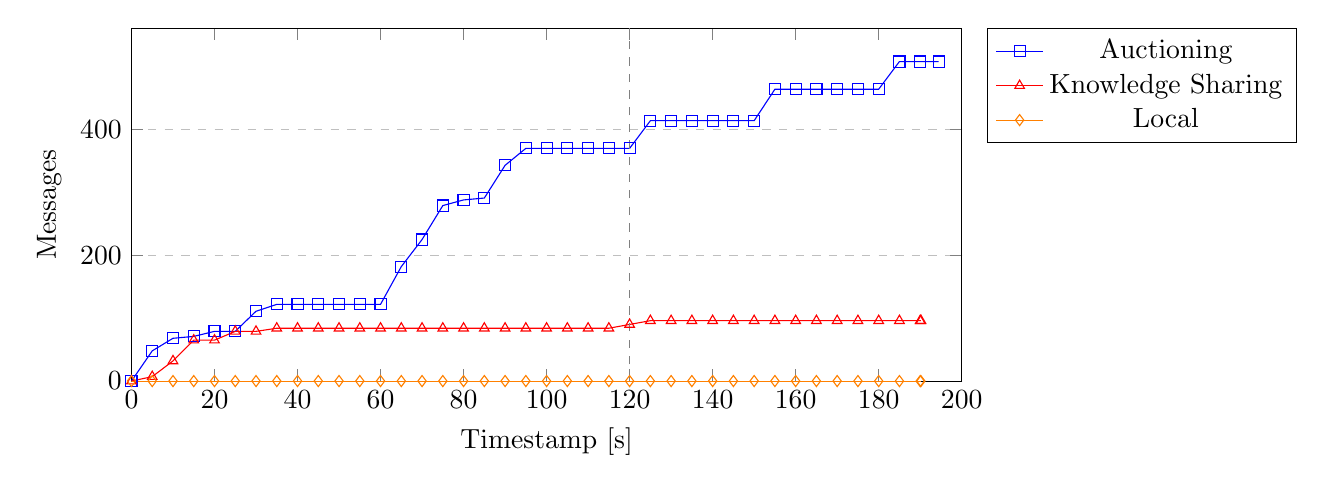
\begin{tikzpicture}
\begin{axis}[
    xlabel={Timestamp [s]},
    ylabel={Messages},
    xmin=0, xmax=200000,
    ymin=0, ymax=561,
    legend pos=outer north east,
    ymajorgrids=true,
    grid style=dashed,
    width=\textwidth,
    height=0.5\textwidth,
    scaled x ticks=base 10:-3,
    xtick scale label code/.code={}
]

	\addplot[color=blue,mark=square] coordinates {
        (0,0)(5000,48)(10000,68)(15000,71)(20000,79)(25000,79)(30000,111)(35000,122)(40000,122)(45000,122)(50000,122)(55000,122)(60000,122)(65000,182)(70000,225)(75000,279)(80000,288)(85000,291)(90000,343)(95000,370)(100000,370)(105000,370)(110000,370)(115000,370)(120000,370)(125000,414)(130000,414)(135000,414)(140000,414)(145000,414)(150000,414)(155000,464)(160000,464)(165000,464)(170000,464)(175000,464)(180000,464)(185000,508)(190000,508)(194440,508)
    };
    \addlegendentry{Auctioning}
	\addplot[color=red,mark=triangle] coordinates {
        (0,0)(5000,7)(10000,32)(15000,65)(20000,65)(25000,79)(30000,79)(35000,84)(40000,84)(45000,84)(50000,84)(55000,84)(60000,84)(65000,84)(70000,84)(75000,84)(80000,84)(85000,84)(90000,84)(95000,84)(100000,84)(105000,84)(110000,84)(115000,84)(120000,90)(125000,96)(130000,96)(135000,96)(140000,96)(145000,96)(150000,96)(155000,96)(160000,96)(165000,96)(170000,96)(175000,96)(180000,96)(185000,96)(190000,96)(190192,96)
    };
    \addlegendentry{Knowledge Sharing}
	\addplot[color=orange,mark=diamond] coordinates {
        (0,0)(5000,0)(10000,0)(15000,0)(20000,0)(25000,0)(30000,0)(35000,0)(40000,0)(45000,0)(50000,0)(55000,0)(60000,0)(65000,0)(70000,0)(75000,0)(80000,0)(85000,0)(90000,0)(95000,0)(100000,0)(105000,0)(110000,0)(115000,0)(120000,0)(125000,0)(130000,0)(135000,0)(140000,0)(145000,0)(150000,0)(155000,0)(160000,0)(165000,0)(170000,0)(175000,0)(180000,0)(185000,0)(190000,0)(190162,0)
    };
    \addlegendentry{Local}

	\addplot[color=gray, dashed,] coordinates {(120000,0) (120000,561)};


\end{axis}
\end{tikzpicture}
    \caption{Graph showing the total amount of messages sent between agents in the risk introduction scenario.}
    \label{fig:messages-risk-introduction}
\end{figure}

Figure \ref{fig:messages-risk-introduction} shows a graph similar to figure \ref{fig:messages-no-change}. The auctioning agent sends the most messages, followed by the knowledge-sharing agent. The local-agent sends no messages. We see that after the $120$ seconds mark, both the auctioning and knowledge-sharing agents send a few more messages around. This is to be expected as the agents detect a change in their properties, and start sharing this information with other agents.

\begin{figure}[H]
    \centering
    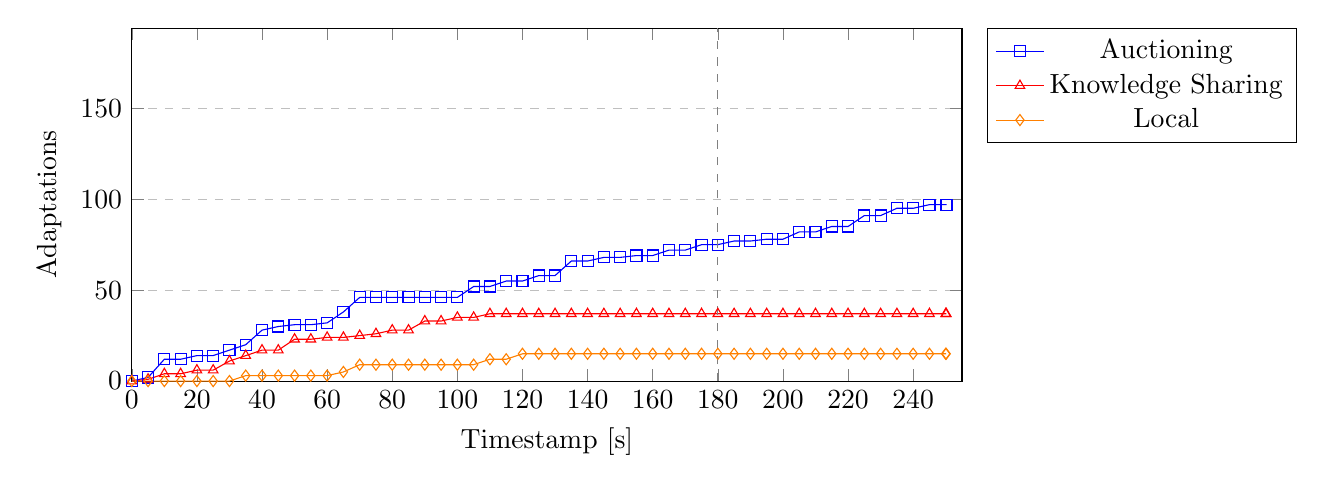
\begin{tikzpicture}
\begin{axis}[
    xlabel={Timestamp [s]},
    ylabel={Adaptations},
    xmin=0, xmax=255000,
    ymin=0, ymax=194,
    legend pos=outer north east,
    ymajorgrids=true,
    grid style=dashed,
    width=\textwidth,
    height=0.5\textwidth,
    scaled x ticks=base 10:-3,
    xtick scale label code/.code={}
]

	\addplot[color=blue,mark=square] coordinates {
        (0,0)(5000,2)(10000,12)(15000,12)(20000,14)(25000,14)(30000,17)(35000,20)(40000,28)(45000,30)(50000,31)(55000,31)(60000,32)(65000,38)(70000,46)(75000,46)(80000,46)(85000,46)(90000,46)(95000,46)(100000,46)(105000,52)(110000,52)(115000,55)(120000,55)(125000,58)(130000,58)(135000,66)(140000,66)(145000,68)(150000,68)(155000,69)(160000,69)(165000,72)(170000,72)(175000,75)(180000,75)(185000,77)(190000,77)(195000,78)(200000,78)(205000,82)(210000,82)(215000,85)(220000,85)(225000,91)(230000,91)(235000,95)(240000,95)(245000,97)(250000,97)(250288,97)
    };
    \addlegendentry{Auctioning}
	\addplot[color=red,mark=triangle] coordinates {
        (0,0)(5000,1)(10000,4)(15000,4)(20000,6)(25000,6)(30000,11)(35000,14)(40000,17)(45000,17)(50000,23)(55000,23)(60000,24)(65000,24)(70000,25)(75000,26)(80000,28)(85000,28)(90000,33)(95000,33)(100000,35)(105000,35)(110000,37)(115000,37)(120000,37)(125000,37)(130000,37)(135000,37)(140000,37)(145000,37)(150000,37)(155000,37)(160000,37)(165000,37)(170000,37)(175000,37)(180000,37)(185000,37)(190000,37)(195000,37)(200000,37)(205000,37)(210000,37)(215000,37)(220000,37)(225000,37)(230000,37)(235000,37)(240000,37)(245000,37)(250000,37)(250159,37)
    };
    \addlegendentry{Knowledge Sharing}
	\addplot[color=orange,mark=diamond] coordinates {
        (0,0)(5000,0)(10000,0)(15000,0)(20000,0)(25000,0)(30000,0)(35000,3)(40000,3)(45000,3)(50000,3)(55000,3)(60000,3)(65000,5)(70000,9)(75000,9)(80000,9)(85000,9)(90000,9)(95000,9)(100000,9)(105000,9)(110000,12)(115000,12)(120000,15)(125000,15)(130000,15)(135000,15)(140000,15)(145000,15)(150000,15)(155000,15)(160000,15)(165000,15)(170000,15)(175000,15)(180000,15)(185000,15)(190000,15)(195000,15)(200000,15)(205000,15)(210000,15)(215000,15)(220000,15)(225000,15)(230000,15)(235000,15)(240000,15)(245000,15)(250000,15)(250135,15)
    };
    \addlegendentry{Local}

	\addplot[color=gray, dashed,] coordinates {(180000,0) (180000,194)};


\end{axis}
\end{tikzpicture}
    \caption{Graph showing the total amount of adaptations applied by agents in the risk introduction scenario.}
    \label{fig:proposals-risk-introduction}
\end{figure}

When the risk is introduced after $120$ seconds, we can see in Figure \ref{fig:proposals-risk-introduction} that a few new adaptations are applied. This is in line with the damage graph in figure \ref{fig:overall-damage-inroduce-risk}.

\begin{figure}[H]
    \centering
        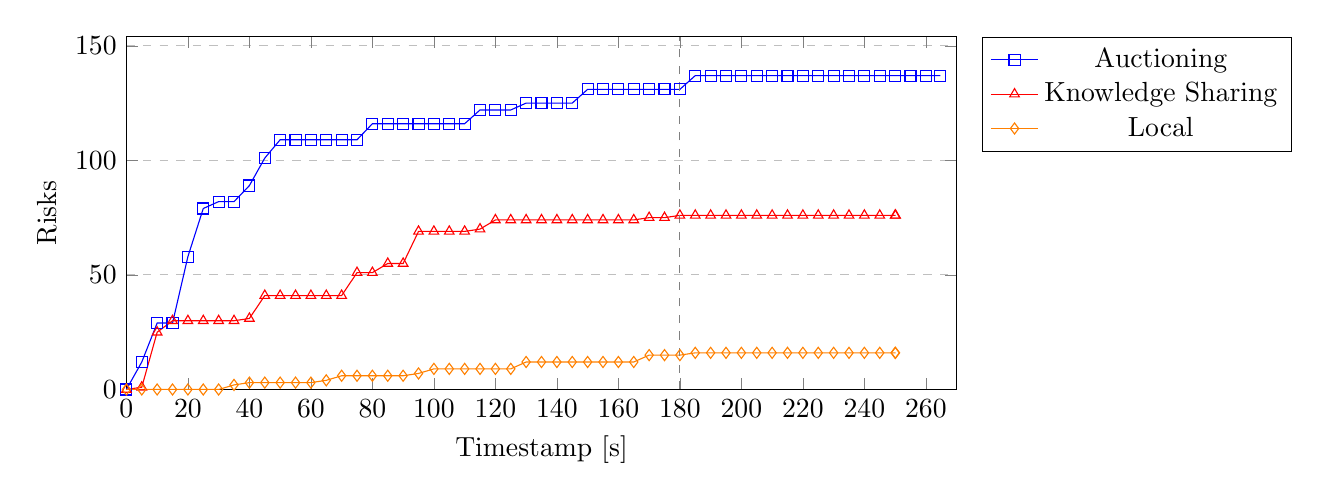
\begin{tikzpicture}
\begin{axis}[
    xlabel={Timestamp [s]},
    ylabel={Risks},
    xmin=0, xmax=270000,
    ymin=0, ymax=154,
    legend pos=outer north east,
    ymajorgrids=true,
    grid style=dashed,
    width=\textwidth,
    height=0.5\textwidth,
    scaled x ticks=base 10:-3,
    xtick scale label code/.code={}
]

	\addplot[color=blue,mark=square] coordinates {
        (0,0)(5000,12)(10000,29)(15000,29)(20000,58)(25000,79)(30000,82)(35000,82)(40000,89)(45000,101)(50000,109)(55000,109)(60000,109)(65000,109)(70000,109)(75000,109)(80000,116)(85000,116)(90000,116)(95000,116)(100000,116)(105000,116)(110000,116)(115000,122)(120000,122)(125000,122)(130000,125)(135000,125)(140000,125)(145000,125)(150000,131)(155000,131)(160000,131)(165000,131)(170000,131)(175000,131)(180000,131)(185000,137)(190000,137)(195000,137)(200000,137)(205000,137)(210000,137)(215000,137)(220000,137)(225000,137)(230000,137)(235000,137)(240000,137)(245000,137)(250000,137)(255000,137)(260000,137)(264723,137)
    };
    \addlegendentry{Auctioning}
	\addplot[color=red,mark=triangle] coordinates {
        (0,0)(5000,1)(10000,25)(15000,30)(20000,30)(25000,30)(30000,30)(35000,30)(40000,31)(45000,41)(50000,41)(55000,41)(60000,41)(65000,41)(70000,41)(75000,51)(80000,51)(85000,55)(90000,55)(95000,69)(100000,69)(105000,69)(110000,69)(115000,70)(120000,74)(125000,74)(130000,74)(135000,74)(140000,74)(145000,74)(150000,74)(155000,74)(160000,74)(165000,74)(170000,75)(175000,75)(180000,76)(185000,76)(190000,76)(195000,76)(200000,76)(205000,76)(210000,76)(215000,76)(220000,76)(225000,76)(230000,76)(235000,76)(240000,76)(245000,76)(250000,76)(250156,76)
    };
    \addlegendentry{Knowledge Sharing}
	\addplot[color=orange,mark=diamond] coordinates {
        (0,0)(5000,0)(10000,0)(15000,0)(20000,0)(25000,0)(30000,0)(35000,2)(40000,3)(45000,3)(50000,3)(55000,3)(60000,3)(65000,4)(70000,6)(75000,6)(80000,6)(85000,6)(90000,6)(95000,7)(100000,9)(105000,9)(110000,9)(115000,9)(120000,9)(125000,9)(130000,12)(135000,12)(140000,12)(145000,12)(150000,12)(155000,12)(160000,12)(165000,12)(170000,15)(175000,15)(180000,15)(185000,16)(190000,16)(195000,16)(200000,16)(205000,16)(210000,16)(215000,16)(220000,16)(225000,16)(230000,16)(235000,16)(240000,16)(245000,16)(250000,16)(250126,16)
    };
    \addlegendentry{Local}

	\addplot[color=gray, dashed,] coordinates {(180000,0) (180000,154)};


\end{axis}
\end{tikzpicture}
    \caption{Graph showing the number of unique risks detected by agents in the risk introduction scenario.}
    \label{fig:risk-count-risk-introduction}
\end{figure}

When we look at figure \ref{fig:risk-count-risk-introduction} we can see that the knowledge-sharing agent detects the most risks, followed by the auctioning agent. The local-agent detects the least amount of risks, at only $10\%$ of the risks found by the knowledge-sharing agent. We would expect a comparable result between the auctioning and knowledge-sharing agents, however this is not the case. This is likely due to the fact that in the knowledge-sharing setup agents apply multiple adaptations in parallel. This causes the knowledge bases to change more rapidly, which could cause the agents to detect more risks. This is explained in more detail in subsection \ref{ssec:metrics}.

\begin{figure}[H]
    \centering
        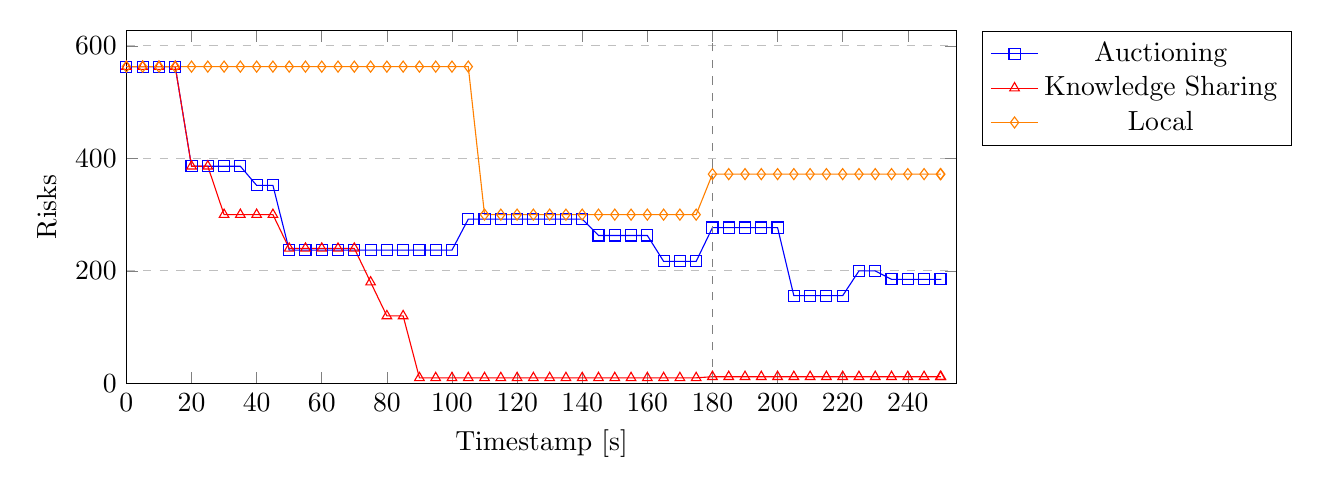
\begin{tikzpicture}
\begin{axis}[
    xlabel={Timestamp [s]},
    ylabel={Risks},
    xmin=0, xmax=255000,
    ymin=0, ymax=627,
    legend pos=outer north east,
    ymajorgrids=true,
    grid style=dashed,
    width=\textwidth,
    height=0.5\textwidth,
    scaled x ticks=base 10:-3,
    xtick scale label code/.code={}
]

	\addplot[color=blue,mark=square] coordinates {
        (0,563)(5000,563)(10000,563)(15000,563)(20000,386)(25000,386)(30000,386)(35000,386)(40000,352)(45000,352)(50000,237)(55000,237)(60000,237)(65000,237)(70000,237)(75000,237)(80000,237)(85000,237)(90000,237)(95000,237)(100000,237)(105000,292)(110000,292)(115000,292)(120000,292)(125000,292)(130000,292)(135000,292)(140000,292)(145000,263)(150000,263)(155000,263)(160000,263)(165000,217)(170000,217)(175000,217)(180000,277)(185000,277)(190000,277)(195000,277)(200000,277)(205000,156)(210000,156)(215000,156)(220000,156)(225000,200)(230000,200)(235000,185)(240000,185)(245000,185)(250000,185)(250288,185)
    };
    \addlegendentry{Auctioning}
	\addplot[color=red,mark=triangle] coordinates {
        (0,563)(5000,563)(10000,563)(15000,563)(20000,386)(25000,386)(30000,300)(35000,300)(40000,300)(45000,300)(50000,240)(55000,240)(60000,240)(65000,240)(70000,240)(75000,180)(80000,120)(85000,120)(90000,10)(95000,10)(100000,10)(105000,10)(110000,10)(115000,10)(120000,10)(125000,10)(130000,10)(135000,10)(140000,10)(145000,10)(150000,10)(155000,10)(160000,10)(165000,10)(170000,10)(175000,10)(180000,12)(185000,12)(190000,12)(195000,12)(200000,12)(205000,12)(210000,12)(215000,12)(220000,12)(225000,12)(230000,12)(235000,12)(240000,12)(245000,12)(250000,12)(250159,12)
    };
    \addlegendentry{Knowledge Sharing}
	\addplot[color=orange,mark=diamond] coordinates {
        (0,563)(5000,563)(10000,563)(15000,563)(20000,563)(25000,563)(30000,563)(35000,563)(40000,563)(45000,563)(50000,563)(55000,563)(60000,563)(65000,563)(70000,563)(75000,563)(80000,563)(85000,563)(90000,563)(95000,563)(100000,563)(105000,563)(110000,300)(115000,300)(120000,300)(125000,300)(130000,300)(135000,300)(140000,300)(145000,300)(150000,300)(155000,300)(160000,300)(165000,300)(170000,300)(175000,300)(180000,372)(185000,372)(190000,372)(195000,372)(200000,372)(205000,372)(210000,372)(215000,372)(220000,372)(225000,372)(230000,372)(235000,372)(240000,372)(245000,372)(250000,372)(250135,372)
    };
    \addlegendentry{Local}

	\addplot[color=gray, dashed,] coordinates {(180000,0) (180000,627)};


\end{axis}
\end{tikzpicture}
    \caption{Graph showing the number of remaining risks in the infrastructure in the risk introduction scenario.}
    \label{fig:risk-remaining-risk-introduction}
\end{figure}

\add{Write}

\begin{figure}[H]
    \centering
        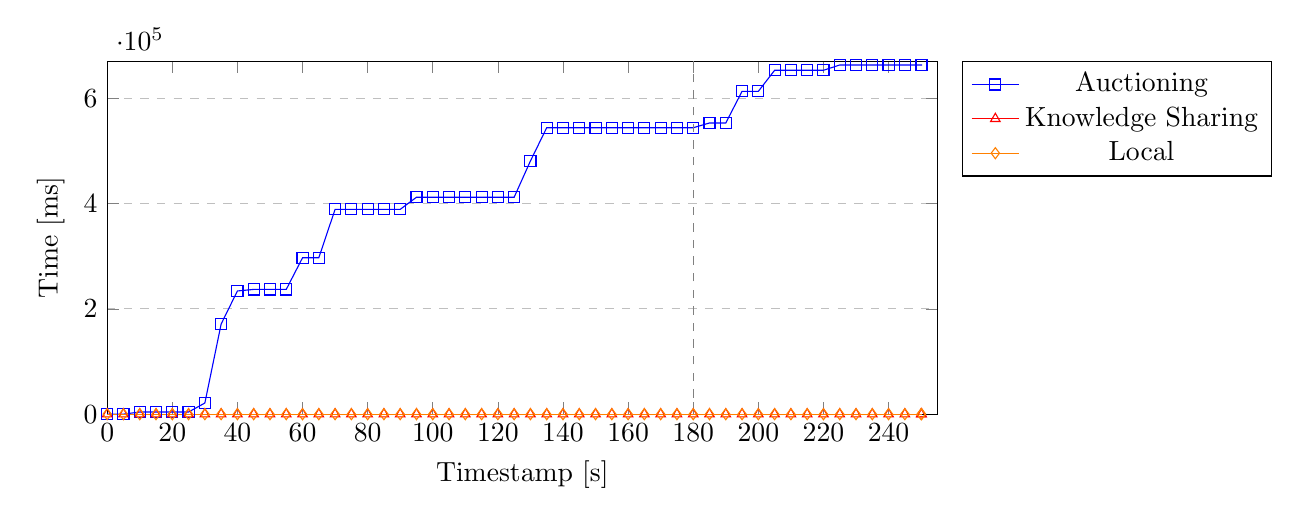
\begin{tikzpicture}
\begin{axis}[
    xlabel={Timestamp [s]},
    ylabel={Time [ms]},
    xmin=0, xmax=255000,
    ymin=0, ymax=670067,
    legend pos=outer north east,
    ymajorgrids=true,
    grid style=dashed,
    width=\textwidth,
    height=0.5\textwidth,
    scaled x ticks=base 10:-3,
    xtick scale label code/.code={}
]

	\addplot[color=blue,mark=square] coordinates {
        (0,0)(5000,64)(10000,4143)(15000,4143)(20000,4143)(25000,4143)(30000,21179)(35000,171183)(40000,233978)(45000,236929)(50000,236929)(55000,236929)(60000,297046)(65000,297049)(70000,388980)(75000,388980)(80000,388980)(85000,388980)(90000,388980)(95000,411980)(100000,411980)(105000,411980)(110000,411980)(115000,411980)(120000,411980)(125000,411980)(130000,480905)(135000,543951)(140000,543951)(145000,543951)(150000,543951)(155000,543958)(160000,543958)(165000,543962)(170000,543962)(175000,543962)(180000,543962)(185000,553054)(190000,553054)(195000,613073)(200000,613073)(205000,653079)(210000,653079)(215000,653087)(220000,653087)(225000,663101)(230000,663101)(235000,663101)(240000,663101)(245000,663101)(250000,663101)(250288,663101)
    };
    \addlegendentry{Auctioning}
	\addplot[color=red,mark=triangle] coordinates {
        (0,0)(5000,0)(10000,0)(15000,0)(20000,0)(25000,0)(30000,0)(35000,0)(40000,0)(45000,0)(50000,0)(55000,0)(60000,0)(65000,0)(70000,0)(75000,0)(80000,0)(85000,0)(90000,0)(95000,0)(100000,0)(105000,0)(110000,0)(115000,0)(120000,0)(125000,0)(130000,0)(135000,0)(140000,0)(145000,0)(150000,0)(155000,0)(160000,0)(165000,0)(170000,0)(175000,0)(180000,0)(185000,0)(190000,0)(195000,0)(200000,0)(205000,0)(210000,0)(215000,0)(220000,0)(225000,0)(230000,0)(235000,0)(240000,0)(245000,0)(250000,0)(250159,0)
    };
    \addlegendentry{Knowledge Sharing}
	\addplot[color=orange,mark=diamond] coordinates {
        (0,0)(5000,0)(10000,0)(15000,0)(20000,0)(25000,0)(30000,0)(35000,0)(40000,0)(45000,0)(50000,0)(55000,0)(60000,0)(65000,0)(70000,0)(75000,0)(80000,0)(85000,0)(90000,0)(95000,0)(100000,0)(105000,0)(110000,0)(115000,0)(120000,0)(125000,0)(130000,0)(135000,0)(140000,0)(145000,0)(150000,0)(155000,0)(160000,0)(165000,0)(170000,0)(175000,0)(180000,0)(185000,0)(190000,0)(195000,0)(200000,0)(205000,0)(210000,0)(215000,0)(220000,0)(225000,0)(230000,0)(235000,0)(240000,0)(245000,0)(250000,0)(250135,0)
    };
    \addlegendentry{Local}

	\addplot[color=gray, dashed,] coordinates {(180000,0) (180000,670067)};


\end{axis}
\end{tikzpicture}
    \caption{Graph showing the sum of time spent auctioning by agents in the risk introduction scenario.}
    \label{fig:auctioning-time-risk-introduction}
\end{figure}

As with figure \ref{fig:auctioning-time-no-change}, we see in figure \ref{fig:adapting-time-risk-introduction} that only the auctioning agent spends time auctioning. The knowledge-sharing agent spends no time auctioning, as it does not have this feature-set. After the $120$ seconds mark we see that the auctioning agent spends more time auctioning, which is a result of the risk being introduced.

\begin{figure}[H]
    \centering
        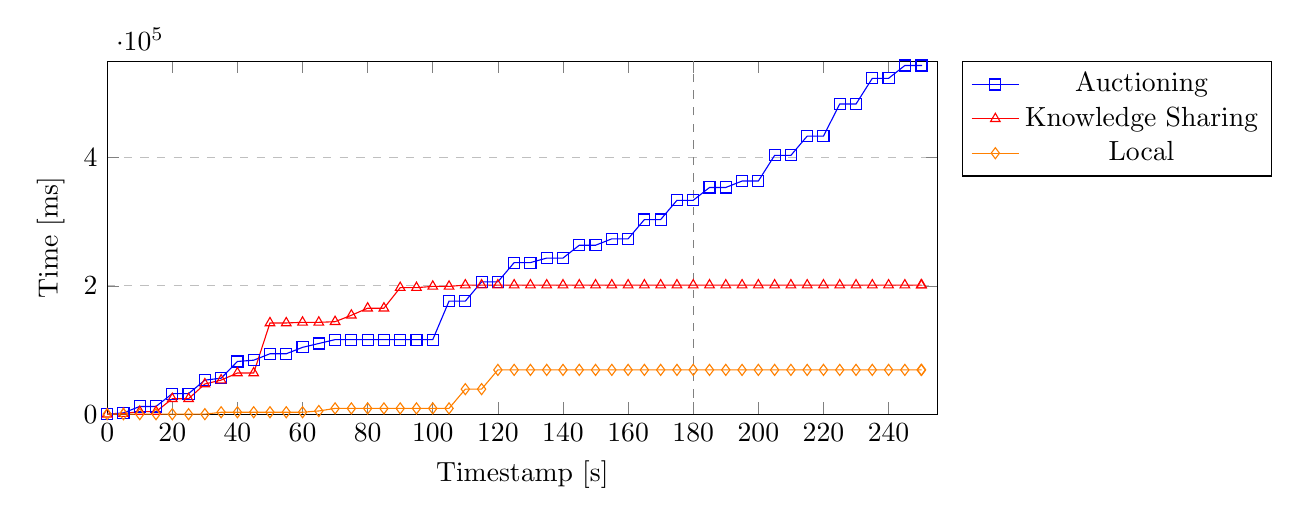
\begin{tikzpicture}
\begin{axis}[
    xlabel={Timestamp [s]},
    ylabel={Time [ms]},
    xmin=0, xmax=255000,
    ymin=0, ymax=550055,
    legend pos=outer north east,
    ymajorgrids=true,
    grid style=dashed,
    width=\textwidth,
    height=0.5\textwidth,
    scaled x ticks=base 10:-3,
    xtick scale label code/.code={}
]

	\addplot[color=blue,mark=square] coordinates {
        (0,0)(5000,2012)(10000,12058)(15000,12058)(20000,32063)(25000,32063)(30000,53081)(35000,56105)(40000,82157)(45000,84176)(50000,94183)(55000,94183)(60000,104190)(65000,110193)(70000,116237)(75000,116237)(80000,116237)(85000,116237)(90000,116237)(95000,116237)(100000,116237)(105000,176271)(110000,176271)(115000,206296)(120000,206296)(125000,236320)(130000,236320)(135000,243360)(140000,243360)(145000,263364)(150000,263364)(155000,273368)(160000,273368)(165000,303394)(170000,303394)(175000,333415)(180000,333415)(185000,353427)(190000,353427)(195000,363436)(200000,363436)(205000,403461)(210000,403461)(215000,433478)(220000,433478)(225000,483523)(230000,483523)(235000,523553)(240000,523553)(245000,543563)(250000,543563)(250288,543563)
    };
    \addlegendentry{Auctioning}
	\addplot[color=red,mark=triangle] coordinates {
        (0,0)(5000,1005)(10000,4021)(15000,4021)(20000,24028)(25000,24028)(30000,47052)(35000,53154)(40000,64163)(45000,64163)(50000,142192)(55000,142192)(60000,143196)(65000,143196)(70000,144197)(75000,154200)(80000,165206)(85000,165206)(90000,197224)(95000,197224)(100000,199232)(105000,199232)(110000,201240)(115000,201240)(120000,201240)(125000,201240)(130000,201240)(135000,201240)(140000,201240)(145000,201240)(150000,201240)(155000,201240)(160000,201240)(165000,201240)(170000,201240)(175000,201240)(180000,201240)(185000,201240)(190000,201240)(195000,201240)(200000,201240)(205000,201240)(210000,201240)(215000,201240)(220000,201240)(225000,201240)(230000,201240)(235000,201240)(240000,201240)(245000,201240)(250000,201240)(250159,201240)
    };
    \addlegendentry{Knowledge Sharing}
	\addplot[color=orange,mark=diamond] coordinates {
        (0,0)(5000,0)(10000,0)(15000,0)(20000,0)(25000,0)(30000,0)(35000,3017)(40000,3017)(45000,3017)(50000,3017)(55000,3017)(60000,3017)(65000,5025)(70000,9035)(75000,9035)(80000,9035)(85000,9035)(90000,9035)(95000,9035)(100000,9035)(105000,9035)(110000,39044)(115000,39044)(120000,69058)(125000,69058)(130000,69058)(135000,69058)(140000,69058)(145000,69058)(150000,69058)(155000,69058)(160000,69058)(165000,69058)(170000,69058)(175000,69058)(180000,69058)(185000,69058)(190000,69058)(195000,69058)(200000,69058)(205000,69058)(210000,69058)(215000,69058)(220000,69058)(225000,69058)(230000,69058)(235000,69058)(240000,69058)(245000,69058)(250000,69058)(250135,69058)
    };
    \addlegendentry{Local}

	\addplot[color=gray, dashed,] coordinates {(180000,0) (180000,550055)};


\end{axis}
\end{tikzpicture}
    \caption{Graph showing the sum of time spent adapting by agents in the risk introduction scenario.}
    \label{fig:adapting-time-risk-introduction}
\end{figure}

Figure \ref{fig:adapting-time-risk-introduction} shows that the knowledge-sharing agent is still spending more time adapting compared to the auctioning agent. Compared to figure \ref{fig:adapting-time-no-change} we see that the agents are all spending roughly the same amount of time adapting, until the $120$ second mark. After this time a bump is observable in the graph.

\subsection{Scenario 3: Growing Infrastructure}
\textit{This scenario introduces a new infrastructure node every $30$ seconds. The purpose of this scenario is to see how the system behaves when the infrastructure is growing.}

\begin{figure}[H]
    \centering
    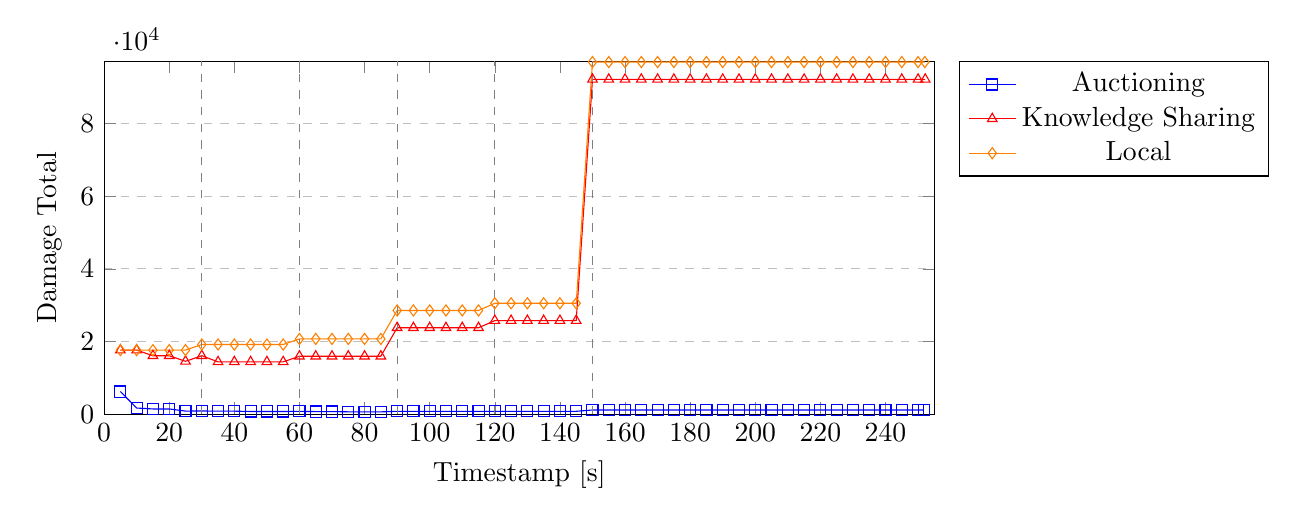
\begin{tikzpicture}
\begin{axis}[
    xlabel={Timestamp [s]},
    ylabel={Damage Total},
    xmin=0, xmax=255000,
    ymin=0, ymax=97097,
    legend pos=outer north east,
    ymajorgrids=true,
    grid style=dashed,
    width=\textwidth,
    height=0.5\textwidth,
    scaled x ticks=base 10:-3,
    xtick scale label code/.code={}
]

	\addplot[color=blue,mark=square] coordinates {
        (5000,6236.51)(10000,1693.70)(15000,1442.78)(20000,1442.78)(25000,857.00)(30000,882.24)(35000,830.70)(40000,830.70)(45000,747.92)(50000,747.92)(55000,747.92)(60000,775.51)(65000,722.54)(70000,722.54)(75000,654.66)(80000,645.84)(85000,645.84)(90000,786.16)(95000,786.16)(100000,786.16)(105000,786.16)(110000,786.16)(115000,786.16)(120000,794.99)(125000,794.99)(130000,794.99)(135000,794.99)(140000,794.99)(145000,794.99)(150000,1153.85)(155000,1153.85)(160000,1153.85)(165000,1153.85)(170000,1153.85)(175000,1153.85)(180000,1153.85)(185000,1153.85)(190000,1153.85)(195000,1153.85)(200000,1153.85)(205000,1153.85)(210000,1153.85)(215000,1153.85)(220000,1153.85)(225000,1153.85)(230000,1153.85)(235000,1153.85)(240000,1153.85)(245000,1153.85)(250000,1153.85)(251808,1153.85)
    };
    \addlegendentry{Auctioning}
	\addplot[color=red,mark=triangle] coordinates {
        (5000,17629.95)(10000,17629.95)(15000,16089.24)(20000,16089.24)(25000,14548.54)(30000,16089.24)(35000,14404.74)(40000,14404.74)(45000,14404.74)(50000,14404.74)(55000,14404.74)(60000,15945.45)(65000,15945.45)(70000,15945.45)(75000,15945.45)(80000,15945.45)(85000,15945.45)(90000,23781.19)(95000,23781.19)(100000,23781.19)(105000,23781.19)(110000,23781.19)(115000,23781.19)(120000,25753.29)(125000,25753.29)(130000,25753.29)(135000,25753.29)(140000,25753.29)(145000,25753.29)(150000,92136.15)(155000,92136.15)(160000,92136.15)(165000,92136.15)(170000,92136.15)(175000,92136.15)(180000,92136.15)(185000,92136.15)(190000,92136.15)(195000,92136.15)(200000,92136.15)(205000,92136.15)(210000,92136.15)(215000,92136.15)(220000,92136.15)(225000,92136.15)(230000,92136.15)(235000,92136.15)(240000,92136.15)(245000,92136.15)(250000,92136.15)(252200,92136.15)
    };
    \addlegendentry{Knowledge Sharing}
	\addplot[color=orange,mark=diamond] coordinates {
        (5000,17629.95)(10000,17629.95)(15000,17629.95)(20000,17629.95)(25000,17629.95)(30000,19170.65)(35000,19170.65)(40000,19170.65)(45000,19170.65)(50000,19170.65)(55000,19170.65)(60000,20711.36)(65000,20711.36)(70000,20711.36)(75000,20711.36)(80000,20711.36)(85000,20711.36)(90000,28547.10)(95000,28547.10)(100000,28547.10)(105000,28547.10)(110000,28547.10)(115000,28547.10)(120000,30519.20)(125000,30519.20)(130000,30519.20)(135000,30519.20)(140000,30519.20)(145000,30519.20)(150000,96902.06)(155000,96902.06)(160000,96902.06)(165000,96902.06)(170000,96902.06)(175000,96902.06)(180000,96902.06)(185000,96902.06)(190000,96902.06)(195000,96902.06)(200000,96902.06)(205000,96902.06)(210000,96902.06)(215000,96902.06)(220000,96902.06)(225000,96902.06)(230000,96902.06)(235000,96902.06)(240000,96902.06)(245000,96902.06)(250000,96902.06)(252076,96902.06)
    };
    \addlegendentry{Local}

	\addplot[color=gray, dashed,] coordinates {(30000,0) (30000,97097)};
	\addplot[color=gray, dashed,] coordinates {(60000,0) (60000,97097)};
	\addplot[color=gray, dashed,] coordinates {(90000,0) (90000,97097)};
	\addplot[color=gray, dashed,] coordinates {(120000,0) (120000,97097)};
	\addplot[color=gray, dashed,] coordinates {(150000,0) (150000,97097)};


\end{axis}
\end{tikzpicture}
    \caption{This graph shows the overall damage of the system in the growing scenario. The damage is shown for each of the three strategies. The vertical lines indicate the time at which a node is introduced.}
    \label{fig:overall-damage-growing}
\end{figure}

From Figure \ref{fig:overall-damage-growing} we see that the auctioning and knowledge-sharing agents are able to keep the damage at a stable level, even though the infrastructure is growing. Only at the end do we see that the agents cannot cope with the increasing damage and does the damage increase. The auctioning agent is keeping the overall damage at the lowest point. This is a good result, as the infrastructure is growing, and the agents are able to keep the damage at a low level. 
As mentioned before, the damage is calculated at a $5000$ms interval. This means that the damage could be higher than the graph shows, as adaptations could be applied within the timeframe. This is the case for the auctioning agent and knowledge-sharing agent, which is observed in the log-files. However, the local-agent does not apply any adaptations during this time, this is visible in the diverging lines at the end of the graph.
 
\begin{figure}[H]
    \centering
    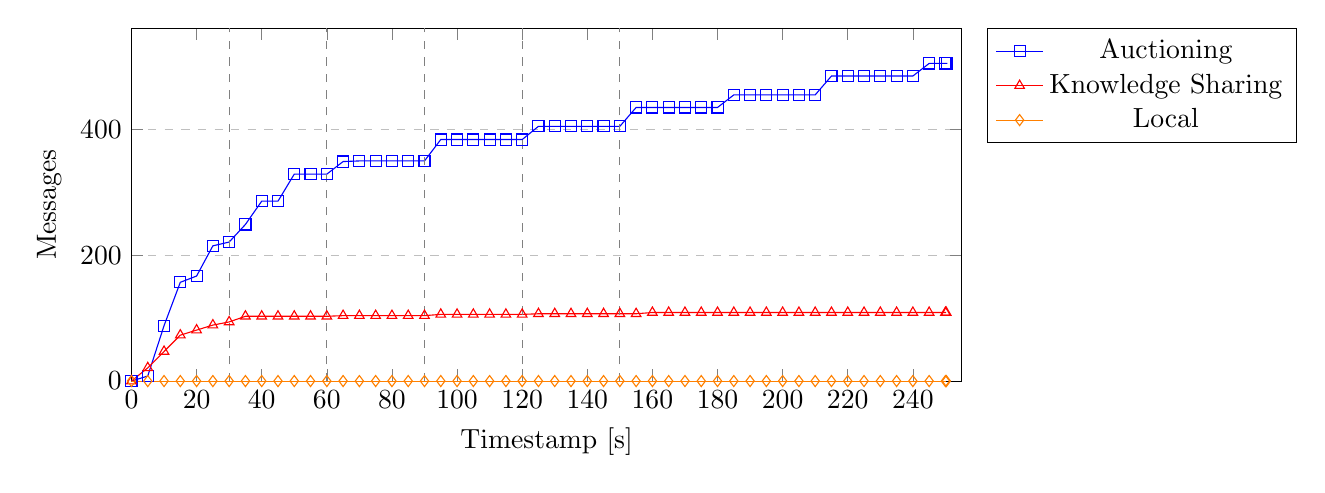
\begin{tikzpicture}
\begin{axis}[
    xlabel={Timestamp [s]},
    ylabel={Messages},
    xmin=0, xmax=255000,
    ymin=0, ymax=561,
    legend pos=outer north east,
    ymajorgrids=true,
    grid style=dashed,
    width=\textwidth,
    height=0.5\textwidth,
    scaled x ticks=base 10:-3,
    xtick scale label code/.code={}
]

	\addplot[color=blue,mark=square] coordinates {
        (0,0)(5000,8)(10000,88)(15000,157)(20000,167)(25000,215)(30000,221)(35000,249)(40000,286)(45000,286)(50000,329)(55000,329)(60000,329)(65000,349)(70000,350)(75000,350)(80000,350)(85000,350)(90000,350)(95000,384)(100000,384)(105000,384)(110000,384)(115000,384)(120000,384)(125000,405)(130000,405)(135000,405)(140000,405)(145000,405)(150000,405)(155000,435)(160000,435)(165000,435)(170000,435)(175000,435)(180000,435)(185000,455)(190000,455)(195000,455)(200000,455)(205000,455)(210000,455)(215000,485)(220000,485)(225000,485)(230000,485)(235000,485)(240000,485)(245000,505)(250000,505)(250569,505)
    };
    \addlegendentry{Auctioning}
	\addplot[color=red,mark=triangle] coordinates {
        (0,0)(5000,21)(10000,47)(15000,73)(20000,81)(25000,89)(30000,94)(35000,103)(40000,103)(45000,103)(50000,103)(55000,103)(60000,103)(65000,104)(70000,104)(75000,104)(80000,104)(85000,104)(90000,104)(95000,106)(100000,106)(105000,106)(110000,106)(115000,106)(120000,106)(125000,107)(130000,107)(135000,107)(140000,107)(145000,107)(150000,107)(155000,107)(160000,109)(165000,109)(170000,109)(175000,109)(180000,109)(185000,109)(190000,109)(195000,109)(200000,109)(205000,109)(210000,109)(215000,109)(220000,109)(225000,109)(230000,109)(235000,109)(240000,109)(245000,109)(250000,109)(250242,109)
    };
    \addlegendentry{Knowledge Sharing}
	\addplot[color=orange,mark=diamond] coordinates {
        (0,0)(5000,0)(10000,0)(15000,0)(20000,0)(25000,0)(30000,0)(35000,0)(40000,0)(45000,0)(50000,0)(55000,0)(60000,0)(65000,0)(70000,0)(75000,0)(80000,0)(85000,0)(90000,0)(95000,0)(100000,0)(105000,0)(110000,0)(115000,0)(120000,0)(125000,0)(130000,0)(135000,0)(140000,0)(145000,0)(150000,0)(155000,0)(160000,0)(165000,0)(170000,0)(175000,0)(180000,0)(185000,0)(190000,0)(195000,0)(200000,0)(205000,0)(210000,0)(215000,0)(220000,0)(225000,0)(230000,0)(235000,0)(240000,0)(245000,0)(250000,0)(250282,0)
    };
    \addlegendentry{Local}

	\addplot[color=gray, dashed,] coordinates {(30000,0) (30000,561)};
	\addplot[color=gray, dashed,] coordinates {(60000,0) (60000,561)};
	\addplot[color=gray, dashed,] coordinates {(90000,0) (90000,561)};
	\addplot[color=gray, dashed,] coordinates {(120000,0) (120000,561)};
	\addplot[color=gray, dashed,] coordinates {(150000,0) (150000,561)};


\end{axis}
\end{tikzpicture}
    \caption{Graph showing the total amount of messages sent between agents in the growing infrastructure scenario.}
    \label{fig:messages-growing}
\end{figure}

Figure \ref{fig:messages-growing} shows that the auctioning agent sends the most messages, followed by the knowledge-sharing agent. The local-agent sends no messages. We see that both the auctioning and knowledge-sharing agents send a few messages around every time a new node is introduced. This is to be expected as the agents detect a change in their properties, and start sharing this information with other agents.

\begin{figure}[H]
    \centering
    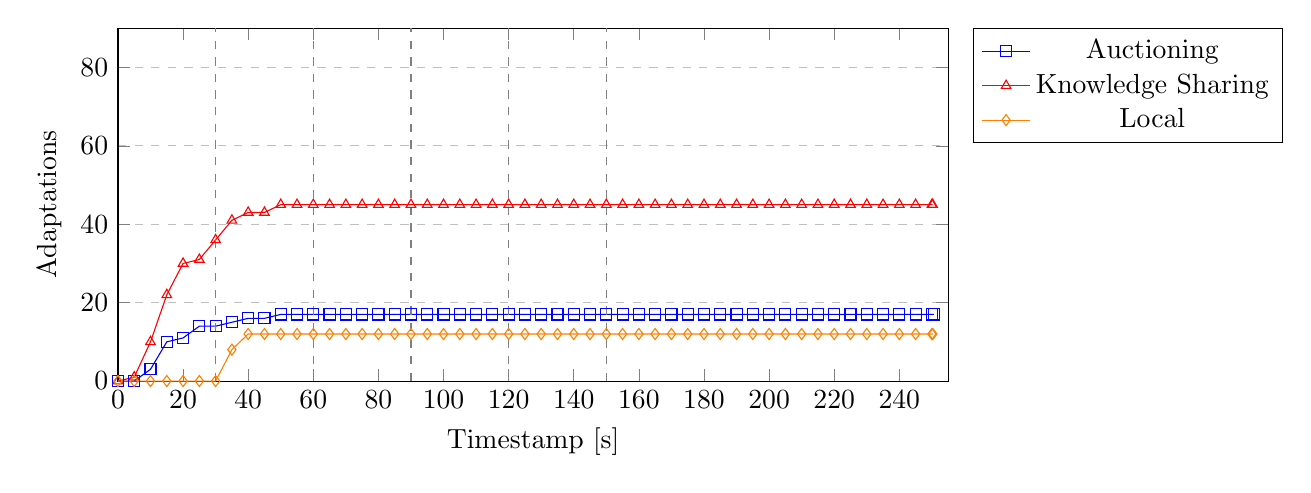
\begin{tikzpicture}
\begin{axis}[
    xlabel={Timestamp [s]},
    ylabel={Adaptations},
    xmin=0, xmax=255000,
    ymin=0, ymax=90,
    legend pos=outer north east,
    ymajorgrids=true,
    grid style=dashed,
    width=\textwidth,
    height=0.5\textwidth,
    scaled x ticks=base 10:-3,
    xtick scale label code/.code={}
]

	\addplot[color=blue,mark=square] coordinates {
        (0,0)(5000,0)(10000,3)(15000,10)(20000,11)(25000,14)(30000,14)(35000,15)(40000,16)(45000,16)(50000,17)(55000,17)(60000,17)(65000,17)(70000,17)(75000,17)(80000,17)(85000,17)(90000,17)(95000,17)(100000,17)(105000,17)(110000,17)(115000,17)(120000,17)(125000,17)(130000,17)(135000,17)(140000,17)(145000,17)(150000,17)(155000,17)(160000,17)(165000,17)(170000,17)(175000,17)(180000,17)(185000,17)(190000,17)(195000,17)(200000,17)(205000,17)(210000,17)(215000,17)(220000,17)(225000,17)(230000,17)(235000,17)(240000,17)(245000,17)(250000,17)(250569,17)
    };
    \addlegendentry{Auctioning}
	\addplot[color=red,mark=triangle] coordinates {
        (0,0)(5000,1)(10000,10)(15000,22)(20000,30)(25000,31)(30000,36)(35000,41)(40000,43)(45000,43)(50000,45)(55000,45)(60000,45)(65000,45)(70000,45)(75000,45)(80000,45)(85000,45)(90000,45)(95000,45)(100000,45)(105000,45)(110000,45)(115000,45)(120000,45)(125000,45)(130000,45)(135000,45)(140000,45)(145000,45)(150000,45)(155000,45)(160000,45)(165000,45)(170000,45)(175000,45)(180000,45)(185000,45)(190000,45)(195000,45)(200000,45)(205000,45)(210000,45)(215000,45)(220000,45)(225000,45)(230000,45)(235000,45)(240000,45)(245000,45)(250000,45)(250242,45)
    };
    \addlegendentry{Knowledge Sharing}
	\addplot[color=orange,mark=diamond] coordinates {
        (0,0)(5000,0)(10000,0)(15000,0)(20000,0)(25000,0)(30000,0)(35000,8)(40000,12)(45000,12)(50000,12)(55000,12)(60000,12)(65000,12)(70000,12)(75000,12)(80000,12)(85000,12)(90000,12)(95000,12)(100000,12)(105000,12)(110000,12)(115000,12)(120000,12)(125000,12)(130000,12)(135000,12)(140000,12)(145000,12)(150000,12)(155000,12)(160000,12)(165000,12)(170000,12)(175000,12)(180000,12)(185000,12)(190000,12)(195000,12)(200000,12)(205000,12)(210000,12)(215000,12)(220000,12)(225000,12)(230000,12)(235000,12)(240000,12)(245000,12)(250000,12)(250282,12)
    };
    \addlegendentry{Local}

	\addplot[color=gray, dashed,] coordinates {(30000,0) (30000,90)};
	\addplot[color=gray, dashed,] coordinates {(60000,0) (60000,90)};
	\addplot[color=gray, dashed,] coordinates {(90000,0) (90000,90)};
	\addplot[color=gray, dashed,] coordinates {(120000,0) (120000,90)};
	\addplot[color=gray, dashed,] coordinates {(150000,0) (150000,90)};


\end{axis}
\end{tikzpicture}
    \caption{Graph showing the total amount of adaptations applied by agents in the growing scenario.}
    \label{fig:proposals-growing}
\end{figure}

As for the adaptations in this experiment, we also see a gradual increase in proposals over time. The local agent is unable to cope with the changes to the infrastructure, and is unable to apply any adaptations. We see that the auctioning agent is slowly applying adaptations, where the knowledge-sharing agent applies them like in quick succession. This is to be expected as the auctioning agent has to negotiate the adaptations, which takes time.

\begin{figure}[H]
    \centering
        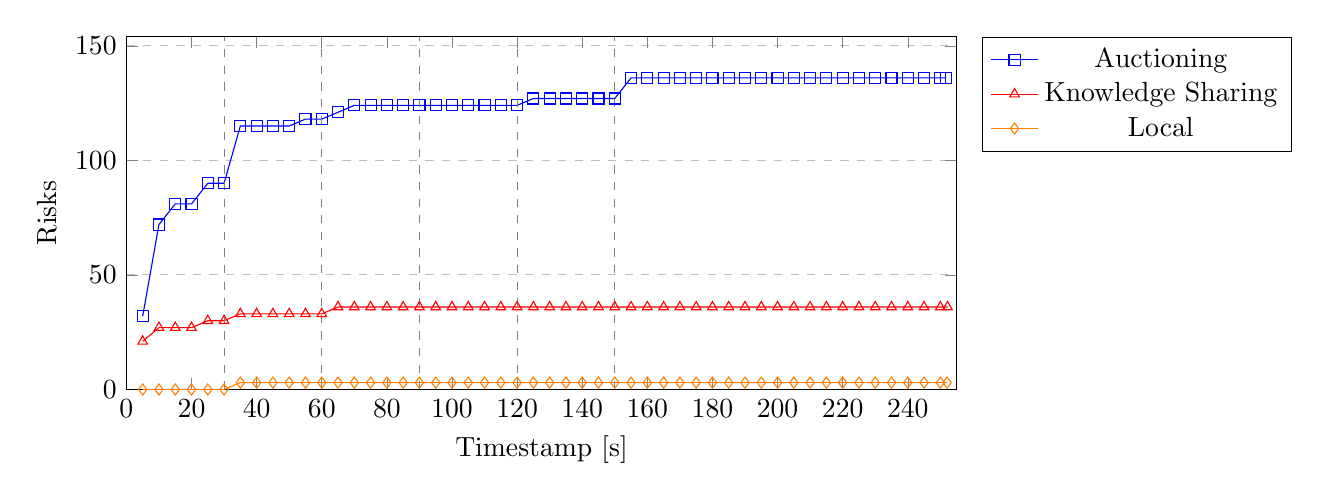
\begin{tikzpicture}
\begin{axis}[
    xlabel={Timestamp [s]},
    ylabel={Risks},
    xmin=0, xmax=255000,
    ymin=0, ymax=154,
    legend pos=outer north east,
    ymajorgrids=true,
    grid style=dashed,
    width=\textwidth,
    height=0.5\textwidth,
    scaled x ticks=base 10:-3,
    xtick scale label code/.code={}
]

	\addplot[color=blue,mark=square] coordinates {
        (5000,32)(10000,72)(15000,81)(20000,81)(25000,90)(30000,90)(35000,115)(40000,115)(45000,115)(50000,115)(55000,118)(60000,118)(65000,121)(70000,124)(75000,124)(80000,124)(85000,124)(90000,124)(95000,124)(100000,124)(105000,124)(110000,124)(115000,124)(120000,124)(125000,127)(130000,127)(135000,127)(140000,127)(145000,127)(150000,127)(155000,136)(160000,136)(165000,136)(170000,136)(175000,136)(180000,136)(185000,136)(190000,136)(195000,136)(200000,136)(205000,136)(210000,136)(215000,136)(220000,136)(225000,136)(230000,136)(235000,136)(240000,136)(245000,136)(250000,136)(251808,136)
    };
    \addlegendentry{Auctioning}
	\addplot[color=red,mark=triangle] coordinates {
        (5000,21)(10000,27)(15000,27)(20000,27)(25000,30)(30000,30)(35000,33)(40000,33)(45000,33)(50000,33)(55000,33)(60000,33)(65000,36)(70000,36)(75000,36)(80000,36)(85000,36)(90000,36)(95000,36)(100000,36)(105000,36)(110000,36)(115000,36)(120000,36)(125000,36)(130000,36)(135000,36)(140000,36)(145000,36)(150000,36)(155000,36)(160000,36)(165000,36)(170000,36)(175000,36)(180000,36)(185000,36)(190000,36)(195000,36)(200000,36)(205000,36)(210000,36)(215000,36)(220000,36)(225000,36)(230000,36)(235000,36)(240000,36)(245000,36)(250000,36)(252200,36)
    };
    \addlegendentry{Knowledge Sharing}
	\addplot[color=orange,mark=diamond] coordinates {
        (5000,0)(10000,0)(15000,0)(20000,0)(25000,0)(30000,0)(35000,3)(40000,3)(45000,3)(50000,3)(55000,3)(60000,3)(65000,3)(70000,3)(75000,3)(80000,3)(85000,3)(90000,3)(95000,3)(100000,3)(105000,3)(110000,3)(115000,3)(120000,3)(125000,3)(130000,3)(135000,3)(140000,3)(145000,3)(150000,3)(155000,3)(160000,3)(165000,3)(170000,3)(175000,3)(180000,3)(185000,3)(190000,3)(195000,3)(200000,3)(205000,3)(210000,3)(215000,3)(220000,3)(225000,3)(230000,3)(235000,3)(240000,3)(245000,3)(250000,3)(252076,3)
    };
    \addlegendentry{Local}

	\addplot[color=gray, dashed,] coordinates {(30000,0) (30000,154)};
	\addplot[color=gray, dashed,] coordinates {(60000,0) (60000,154)};
	\addplot[color=gray, dashed,] coordinates {(90000,0) (90000,154)};
	\addplot[color=gray, dashed,] coordinates {(120000,0) (120000,154)};
	\addplot[color=gray, dashed,] coordinates {(150000,0) (150000,154)};


\end{axis}
\end{tikzpicture}
    \caption{Graph showing the number of unique risks detected by agents in the growing scenario.}
    \label{fig:risk-count-growing}
\end{figure}

Figure \ref{fig:risk-count-growing} show that the knowledge-sharing agent finds the most unique risks, followed by the auctioning agent. The auctioning agent finds only $50\%$ of the risks detected by the knowledge-sharing agent. The local-agent finds the least amount of risks, at only $10\%$ of the risks found by the knowledge-sharing agent. As mentioned in Section \ref{ssec:scenario-2-results}, this is likely due to the fact that in the knowledge-sharing setup agents apply multiple adaptations in parallel. 

\begin{figure}[H]
    \centering
        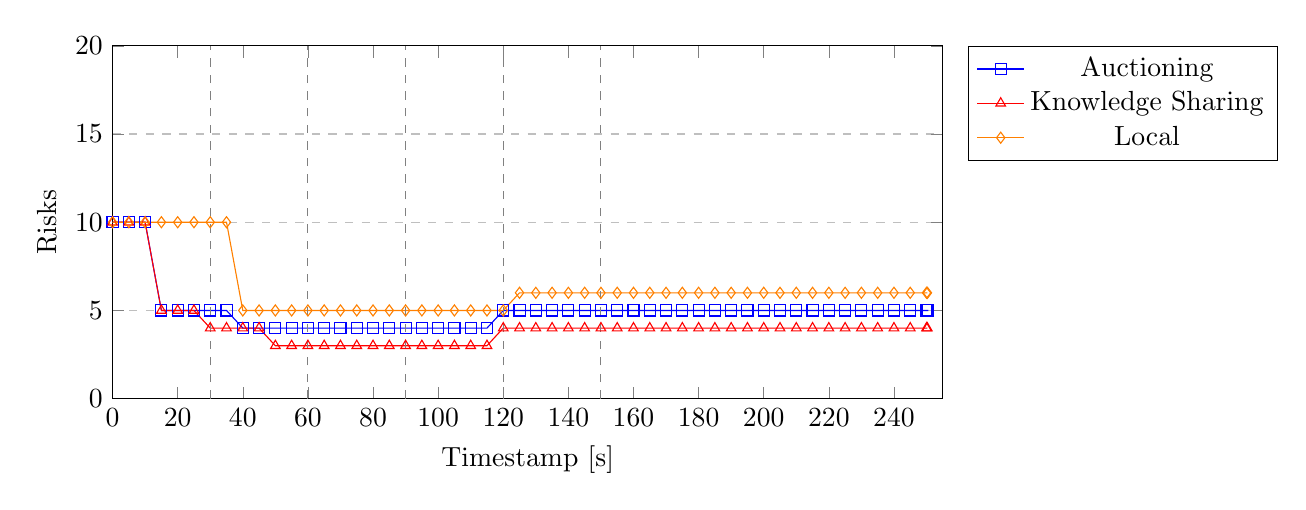
\begin{tikzpicture}
\begin{axis}[
    xlabel={Timestamp [s]},
    ylabel={Risks},
    xmin=0, xmax=255000,
    ymin=0, ymax=20,
    legend pos=outer north east,
    ymajorgrids=true,
    grid style=dashed,
    width=\textwidth,
    height=0.5\textwidth,
    scaled x ticks=base 10:-3,
    xtick scale label code/.code={}
]

	\addplot[color=blue,mark=square] coordinates {
        (0,10)(5000,10)(10000,10)(15000,5)(20000,5)(25000,5)(30000,5)(35000,5)(40000,4)(45000,4)(50000,4)(55000,4)(60000,4)(65000,4)(70000,4)(75000,4)(80000,4)(85000,4)(90000,4)(95000,4)(100000,4)(105000,4)(110000,4)(115000,4)(120000,5)(125000,5)(130000,5)(135000,5)(140000,5)(145000,5)(150000,5)(155000,5)(160000,5)(165000,5)(170000,5)(175000,5)(180000,5)(185000,5)(190000,5)(195000,5)(200000,5)(205000,5)(210000,5)(215000,5)(220000,5)(225000,5)(230000,5)(235000,5)(240000,5)(245000,5)(250000,5)(250569,5)
    };
    \addlegendentry{Auctioning}
	\addplot[color=red,mark=triangle] coordinates {
        (0,10)(5000,10)(10000,10)(15000,5)(20000,5)(25000,5)(30000,4)(35000,4)(40000,4)(45000,4)(50000,3)(55000,3)(60000,3)(65000,3)(70000,3)(75000,3)(80000,3)(85000,3)(90000,3)(95000,3)(100000,3)(105000,3)(110000,3)(115000,3)(120000,4)(125000,4)(130000,4)(135000,4)(140000,4)(145000,4)(150000,4)(155000,4)(160000,4)(165000,4)(170000,4)(175000,4)(180000,4)(185000,4)(190000,4)(195000,4)(200000,4)(205000,4)(210000,4)(215000,4)(220000,4)(225000,4)(230000,4)(235000,4)(240000,4)(245000,4)(250000,4)(250242,4)
    };
    \addlegendentry{Knowledge Sharing}
	\addplot[color=orange,mark=diamond] coordinates {
        (0,10)(5000,10)(10000,10)(15000,10)(20000,10)(25000,10)(30000,10)(35000,10)(40000,5)(45000,5)(50000,5)(55000,5)(60000,5)(65000,5)(70000,5)(75000,5)(80000,5)(85000,5)(90000,5)(95000,5)(100000,5)(105000,5)(110000,5)(115000,5)(120000,5)(125000,6)(130000,6)(135000,6)(140000,6)(145000,6)(150000,6)(155000,6)(160000,6)(165000,6)(170000,6)(175000,6)(180000,6)(185000,6)(190000,6)(195000,6)(200000,6)(205000,6)(210000,6)(215000,6)(220000,6)(225000,6)(230000,6)(235000,6)(240000,6)(245000,6)(250000,6)(250282,6)
    };
    \addlegendentry{Local}

	\addplot[color=gray, dashed,] coordinates {(30000,0) (30000,20)};
	\addplot[color=gray, dashed,] coordinates {(60000,0) (60000,20)};
	\addplot[color=gray, dashed,] coordinates {(90000,0) (90000,20)};
	\addplot[color=gray, dashed,] coordinates {(120000,0) (120000,20)};
	\addplot[color=gray, dashed,] coordinates {(150000,0) (150000,20)};


\end{axis}
\end{tikzpicture}
    \caption{Graph showing the number of remaining risks in the infrastructure in the growing scenario.}
    \label{fig:risk-remaining-growing}
\end{figure}

\add{write}

\begin{figure}[H]
    \centering
        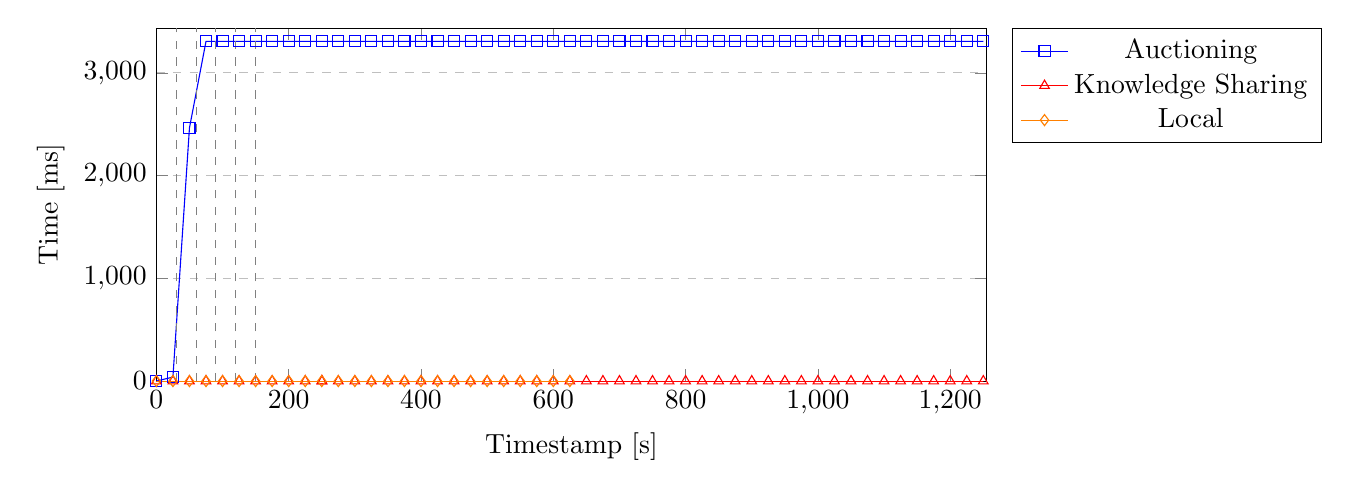
\begin{tikzpicture}
\begin{axis}[
    xlabel={Timestamp [s]},
    ylabel={Time [ms]},
    xmin=0, xmax=1255000,
    ymin=0, ymax=3434,
    legend pos=outer north east,
    ymajorgrids=true,
    grid style=dashed,
    width=\textwidth,
    height=0.5\textwidth,
    scaled x ticks=base 10:-3,
    xtick scale label code/.code={}
]

	\addplot[color=blue,mark=square] coordinates {
        (0,0)(25000,39)(50000,2464)(75000,3306)(100000,3306)(125000,3306)(150000,3306)(175000,3306)(200000,3306)(225000,3306)(250000,3306)(275000,3306)(300000,3306)(325000,3306)(350000,3306)(375000,3306)(400000,3306)(425000,3306)(450000,3306)(475000,3306)(500000,3306)(525000,3306)(550000,3306)(575000,3306)(600000,3306)(625000,3306)(650000,3306)(675000,3306)(700000,3306)(725000,3306)(750000,3306)(775000,3306)(800000,3306)(825000,3306)(850000,3306)(875000,3306)(900000,3306)(925000,3306)(950000,3306)(975000,3306)(1000000,3306)(1025000,3306)(1050000,3306)(1075000,3306)(1100000,3306)(1125000,3306)(1150000,3306)(1175000,3306)(1200000,3306)(1225000,3306)(1250000,3306)(250447,3306)
    };
    \addlegendentry{Auctioning}
	\addplot[color=red,mark=triangle] coordinates {
        (0,0)(25000,0)(50000,0)(75000,0)(100000,0)(125000,0)(150000,0)(175000,0)(200000,0)(225000,0)(250000,0)(275000,0)(300000,0)(325000,0)(350000,0)(375000,0)(400000,0)(425000,0)(450000,0)(475000,0)(500000,0)(525000,0)(550000,0)(575000,0)(600000,0)(625000,0)(650000,0)(675000,0)(700000,0)(725000,0)(750000,0)(775000,0)(800000,0)(825000,0)(850000,0)(875000,0)(900000,0)(925000,0)(950000,0)(975000,0)(1000000,0)(1025000,0)(1050000,0)(1075000,0)(1100000,0)(1125000,0)(1150000,0)(1175000,0)(1200000,0)(1225000,0)(1250000,0)(250418,0)
    };
    \addlegendentry{Knowledge Sharing}
	\addplot[color=orange,mark=diamond] coordinates {
        (0,0)(25000,0)(50000,0)(75000,0)(100000,0)(125000,0)(150000,0)(175000,0)(200000,0)(225000,0)(250000,0)(275000,0)(300000,0)(325000,0)(350000,0)(375000,0)(400000,0)(425000,0)(450000,0)(475000,0)(500000,0)(525000,0)(550000,0)(575000,0)(600000,0)(625000,0)
    };
    \addlegendentry{Local}

	\addplot[color=gray, dashed,] coordinates {(30000,0) (30000,3434)};
	\addplot[color=gray, dashed,] coordinates {(60000,0) (60000,3434)};
	\addplot[color=gray, dashed,] coordinates {(90000,0) (90000,3434)};
	\addplot[color=gray, dashed,] coordinates {(120000,0) (120000,3434)};
	\addplot[color=gray, dashed,] coordinates {(150000,0) (150000,3434)};


\end{axis}
\end{tikzpicture}
    \caption{Graph showing the sum of time spent auctioning by agents in the growing scenario.}
    \label{fig:auctioning-time-growing}
\end{figure}

Figure \ref{fig:auctioning-time-growing} shows an ever growing amount of time spent auctioning. This is in line with the expectations as the agents finds a risk, and then starts an auction. These auctions in the end lead to no proposals/adaptations being applied, as the agents are unable to find a better adaptation. This is visible in the graph as the time spent auctioning increases, but the amount of adaptations from Figure \ref{fig:proposals-growing} stays the same.

\begin{figure}[H]
    \centering
        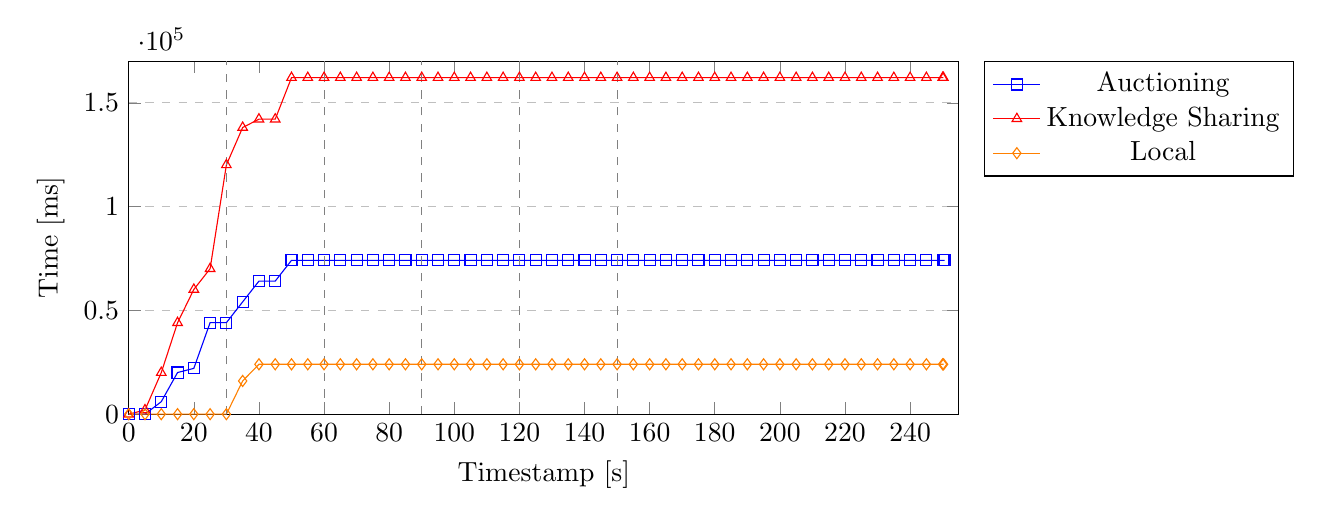
\begin{tikzpicture}
\begin{axis}[
    xlabel={Timestamp [s]},
    ylabel={Time [ms]},
    xmin=0, xmax=255000,
    ymin=0, ymax=170017,
    legend pos=outer north east,
    ymajorgrids=true,
    grid style=dashed,
    width=\textwidth,
    height=0.5\textwidth,
    scaled x ticks=base 10:-3,
    xtick scale label code/.code={}
]

	\addplot[color=blue,mark=square] coordinates {
        (0,0)(5000,0)(10000,6018)(15000,20071)(20000,22078)(25000,44102)(30000,44102)(35000,54111)(40000,64119)(45000,64119)(50000,74128)(55000,74128)(60000,74128)(65000,74128)(70000,74128)(75000,74128)(80000,74128)(85000,74128)(90000,74128)(95000,74128)(100000,74128)(105000,74128)(110000,74128)(115000,74128)(120000,74128)(125000,74128)(130000,74128)(135000,74128)(140000,74128)(145000,74128)(150000,74128)(155000,74128)(160000,74128)(165000,74128)(170000,74128)(175000,74128)(180000,74128)(185000,74128)(190000,74128)(195000,74128)(200000,74128)(205000,74128)(210000,74128)(215000,74128)(220000,74128)(225000,74128)(230000,74128)(235000,74128)(240000,74128)(245000,74128)(250000,74128)(250569,74128)
    };
    \addlegendentry{Auctioning}
	\addplot[color=red,mark=triangle] coordinates {
        (0,0)(5000,2004)(10000,20023)(15000,44059)(20000,60095)(25000,70097)(30000,120113)(35000,138132)(40000,142140)(45000,142140)(50000,162147)(55000,162147)(60000,162147)(65000,162147)(70000,162147)(75000,162147)(80000,162147)(85000,162147)(90000,162147)(95000,162147)(100000,162147)(105000,162147)(110000,162147)(115000,162147)(120000,162147)(125000,162147)(130000,162147)(135000,162147)(140000,162147)(145000,162147)(150000,162147)(155000,162147)(160000,162147)(165000,162147)(170000,162147)(175000,162147)(180000,162147)(185000,162147)(190000,162147)(195000,162147)(200000,162147)(205000,162147)(210000,162147)(215000,162147)(220000,162147)(225000,162147)(230000,162147)(235000,162147)(240000,162147)(245000,162147)(250000,162147)(250242,162147)
    };
    \addlegendentry{Knowledge Sharing}
	\addplot[color=orange,mark=diamond] coordinates {
        (0,0)(5000,0)(10000,0)(15000,0)(20000,0)(25000,0)(30000,0)(35000,16023)(40000,24038)(45000,24038)(50000,24038)(55000,24038)(60000,24038)(65000,24038)(70000,24038)(75000,24038)(80000,24038)(85000,24038)(90000,24038)(95000,24038)(100000,24038)(105000,24038)(110000,24038)(115000,24038)(120000,24038)(125000,24038)(130000,24038)(135000,24038)(140000,24038)(145000,24038)(150000,24038)(155000,24038)(160000,24038)(165000,24038)(170000,24038)(175000,24038)(180000,24038)(185000,24038)(190000,24038)(195000,24038)(200000,24038)(205000,24038)(210000,24038)(215000,24038)(220000,24038)(225000,24038)(230000,24038)(235000,24038)(240000,24038)(245000,24038)(250000,24038)(250282,24038)
    };
    \addlegendentry{Local}

	\addplot[color=gray, dashed,] coordinates {(30000,0) (30000,170017)};
	\addplot[color=gray, dashed,] coordinates {(60000,0) (60000,170017)};
	\addplot[color=gray, dashed,] coordinates {(90000,0) (90000,170017)};
	\addplot[color=gray, dashed,] coordinates {(120000,0) (120000,170017)};
	\addplot[color=gray, dashed,] coordinates {(150000,0) (150000,170017)};


\end{axis}
\end{tikzpicture}
    \caption{Graph showing the sum of time spent adapting by agents in the growing scenario.}
    \label{fig:adapting-time-growing}
\end{figure}

Figure \ref{fig:adapting-time-growing} shows that the knowledge-sharing agent spends the most time adapting, followed by the auctioning agent. We see that compared to Figures \ref{fig:adapting-time-no-change} and \ref{fig:adapting-time-risk-introduction}, that the auctioning agent slowly applies more and more adaptations, whereas the knowledge-sharing agent some of these adaptations applied already. 

\subsection{Scenario 4: Unstable Infrastructure}
\textit{This scenario removes an existing infrastructure node after $30$ seconds, and adds the node back into the infrastructure after another $30$ seconds. This is repeated twice. The purpose of this scenario is to see how the system behaves when the infrastructure (connection) is unstable.}

\begin{figure}[H]
    \centering
    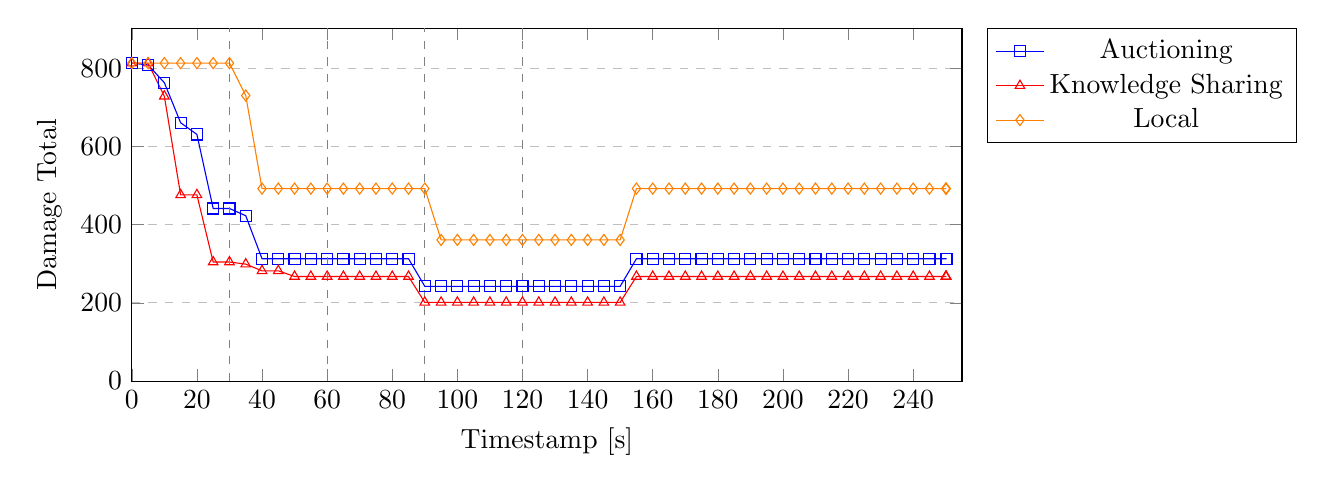
\begin{tikzpicture}
\begin{axis}[
    xlabel={Timestamp [s]},
    ylabel={Damage Total},
    xmin=0, xmax=255000,
    ymin=0, ymax=902,
    legend pos=outer north east,
    ymajorgrids=true,
    grid style=dashed,
    width=\textwidth,
    height=0.5\textwidth,
    scaled x ticks=base 10:-3,
    xtick scale label code/.code={}
]

	\addplot[color=blue,mark=square] coordinates {
        (0,812.71)(5000,808.17)(10000,762.80)(15000,660.38)(20000,630.54)(25000,441.18)(30000,441.18)(35000,422.77)(40000,312.76)(45000,312.76)(50000,312.76)(55000,312.76)(60000,312.76)(65000,312.76)(70000,312.76)(75000,312.76)(80000,312.76)(85000,312.76)(90000,242.13)(95000,242.13)(100000,242.13)(105000,242.13)(110000,242.13)(115000,242.13)(120000,242.13)(125000,242.13)(130000,242.13)(135000,242.13)(140000,242.13)(145000,242.13)(150000,242.13)(155000,312.76)(160000,312.76)(165000,312.76)(170000,312.76)(175000,312.76)(180000,312.76)(185000,312.76)(190000,312.76)(195000,312.76)(200000,312.76)(205000,312.76)(210000,312.76)(215000,312.76)(220000,312.76)(225000,312.76)(230000,312.76)(235000,312.76)(240000,312.76)(245000,312.76)(250000,312.76)(250270,312.76)
    };
    \addlegendentry{Auctioning}
	\addplot[color=red,mark=triangle] coordinates {
        (0,812.71)(5000,812.71)(10000,728.19)(15000,476.06)(20000,476.06)(25000,304.33)(30000,304.33)(35000,298.99)(40000,281.89)(45000,281.89)(50000,267.31)(55000,267.31)(60000,267.31)(65000,267.31)(70000,267.31)(75000,267.31)(80000,267.31)(85000,267.31)(90000,201.16)(95000,201.16)(100000,201.16)(105000,201.16)(110000,201.16)(115000,201.16)(120000,201.16)(125000,201.16)(130000,201.16)(135000,201.16)(140000,201.16)(145000,201.16)(150000,201.16)(155000,267.31)(160000,267.31)(165000,267.31)(170000,267.31)(175000,267.31)(180000,267.31)(185000,267.31)(190000,267.31)(195000,267.31)(200000,267.31)(205000,267.31)(210000,267.31)(215000,267.31)(220000,267.31)(225000,267.31)(230000,267.31)(235000,267.31)(240000,267.31)(245000,267.31)(250000,267.31)(250172,267.31)
    };
    \addlegendentry{Knowledge Sharing}
	\addplot[color=orange,mark=diamond] coordinates {
        (0,812.71)(5000,812.71)(10000,812.71)(15000,812.71)(20000,812.71)(25000,812.71)(30000,812.71)(35000,729.98)(40000,492.04)(45000,492.04)(50000,492.04)(55000,492.04)(60000,492.04)(65000,492.04)(70000,492.04)(75000,492.04)(80000,492.04)(85000,492.04)(90000,492.04)(95000,360.79)(100000,360.79)(105000,360.79)(110000,360.79)(115000,360.79)(120000,360.79)(125000,360.79)(130000,360.79)(135000,360.79)(140000,360.79)(145000,360.79)(150000,360.79)(155000,492.04)(160000,492.04)(165000,492.04)(170000,492.04)(175000,492.04)(180000,492.04)(185000,492.04)(190000,492.04)(195000,492.04)(200000,492.04)(205000,492.04)(210000,492.04)(215000,492.04)(220000,492.04)(225000,492.04)(230000,492.04)(235000,492.04)(240000,492.04)(245000,492.04)(250000,492.04)(250190,492.04)
    };
    \addlegendentry{Local}

	\addplot[color=gray, dashed,] coordinates {(30000,0) (30000,902)};
	\addplot[color=gray, dashed,] coordinates {(60000,0) (60000,902)};
	\addplot[color=gray, dashed,] coordinates {(90000,0) (90000,902)};
	\addplot[color=gray, dashed,] coordinates {(120000,0) (120000,902)};


\end{axis}
\end{tikzpicture}
    \caption{This graph shows the overall damage of the system in the unstable scenario. The damage is shown for each of the three strategies. The vertical lines indicate the time at which a node was removed and added again.}
    \label{fig:overall-damage-unstable}
\end{figure}

From this first Figure \ref{fig:overall-damage-unstable} we see a trend that is similar to the one from the first experiment (Figure \ref{fig:overall-damage-no-change}). The second time a node gets removed and then added, we see a small dip in the graphs. But apart from this there are no \emph{new} risks to mitigate as the properties of the nodes do not change. This is also reflected in Figure \ref{fig:messages-unstable}, where the knowledge-sharing agent does not see any property changes (and thus does not send any messages). The auctioning node does send some messages, as perviously due to the attempts of finding adaptations.

\begin{figure}[H]
    \centering
    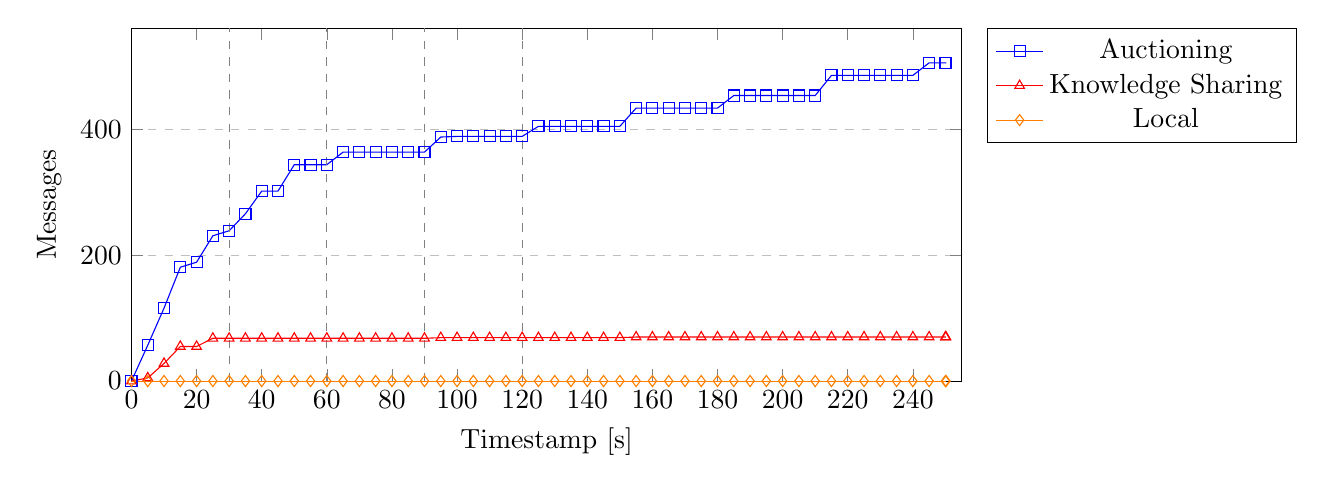
\begin{tikzpicture}
\begin{axis}[
    xlabel={Timestamp [s]},
    ylabel={Messages},
    xmin=0, xmax=255000,
    ymin=0, ymax=561,
    legend pos=outer north east,
    ymajorgrids=true,
    grid style=dashed,
    width=\textwidth,
    height=0.5\textwidth,
    scaled x ticks=base 10:-3,
    xtick scale label code/.code={}
]

	\addplot[color=blue,mark=square] coordinates {
        (0,0)(5000,57)(10000,116)(15000,181)(20000,189)(25000,231)(30000,239)(35000,266)(40000,302)(45000,302)(50000,344)(55000,344)(60000,344)(65000,364)(70000,364)(75000,364)(80000,364)(85000,364)(90000,364)(95000,388)(100000,389)(105000,389)(110000,389)(115000,389)(120000,389)(125000,405)(130000,405)(135000,405)(140000,405)(145000,405)(150000,405)(155000,434)(160000,434)(165000,434)(170000,434)(175000,434)(180000,434)(185000,454)(190000,454)(195000,454)(200000,454)(205000,454)(210000,454)(215000,486)(220000,486)(225000,486)(230000,486)(235000,486)(240000,486)(245000,506)(250000,506)(250270,506)
    };
    \addlegendentry{Auctioning}
	\addplot[color=red,mark=triangle] coordinates {
        (0,0)(5000,5)(10000,28)(15000,55)(20000,55)(25000,68)(30000,68)(35000,68)(40000,68)(45000,68)(50000,68)(55000,68)(60000,68)(65000,68)(70000,68)(75000,68)(80000,68)(85000,68)(90000,68)(95000,69)(100000,69)(105000,69)(110000,69)(115000,69)(120000,69)(125000,69)(130000,69)(135000,69)(140000,69)(145000,69)(150000,69)(155000,70)(160000,70)(165000,70)(170000,70)(175000,70)(180000,70)(185000,70)(190000,70)(195000,70)(200000,70)(205000,70)(210000,70)(215000,70)(220000,70)(225000,70)(230000,70)(235000,70)(240000,70)(245000,70)(250000,70)(250172,70)
    };
    \addlegendentry{Knowledge Sharing}
	\addplot[color=orange,mark=diamond] coordinates {
        (0,0)(5000,0)(10000,0)(15000,0)(20000,0)(25000,0)(30000,0)(35000,0)(40000,0)(45000,0)(50000,0)(55000,0)(60000,0)(65000,0)(70000,0)(75000,0)(80000,0)(85000,0)(90000,0)(95000,0)(100000,0)(105000,0)(110000,0)(115000,0)(120000,0)(125000,0)(130000,0)(135000,0)(140000,0)(145000,0)(150000,0)(155000,0)(160000,0)(165000,0)(170000,0)(175000,0)(180000,0)(185000,0)(190000,0)(195000,0)(200000,0)(205000,0)(210000,0)(215000,0)(220000,0)(225000,0)(230000,0)(235000,0)(240000,0)(245000,0)(250000,0)(250190,0)
    };
    \addlegendentry{Local}

	\addplot[color=gray, dashed,] coordinates {(30000,0) (30000,561)};
	\addplot[color=gray, dashed,] coordinates {(60000,0) (60000,561)};
	\addplot[color=gray, dashed,] coordinates {(90000,0) (90000,561)};
	\addplot[color=gray, dashed,] coordinates {(120000,0) (120000,561)};


\end{axis}
\end{tikzpicture}
    \caption{Graph showing the total amount of messages sent between agents in the unstable scenario.}
    \label{fig:messages-unstable}
\end{figure}

\begin{figure}[H]
    \centering
    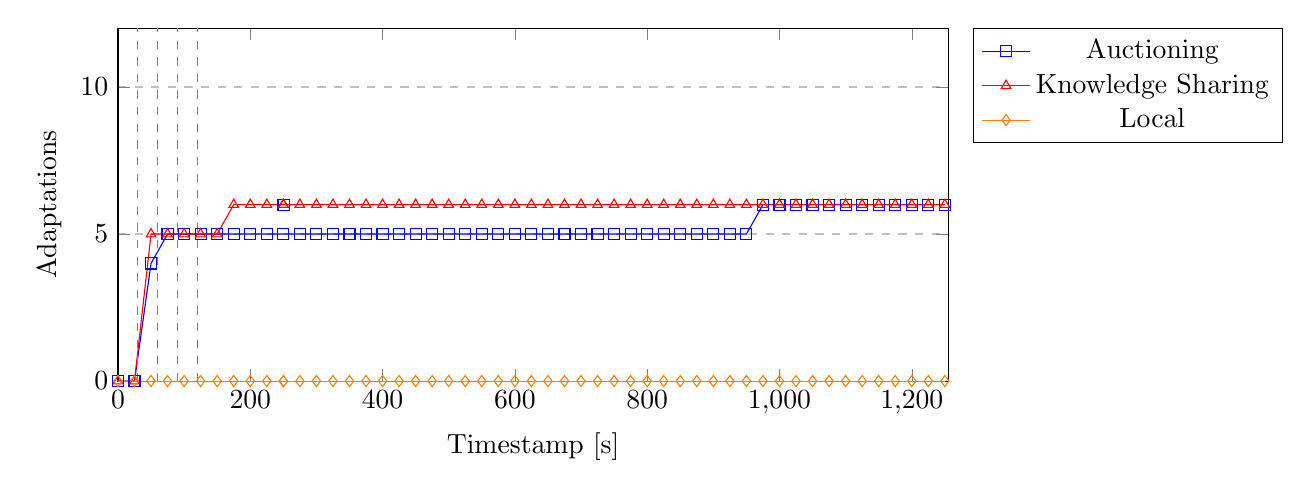
\begin{tikzpicture}
\begin{axis}[
    xlabel={Timestamp [s]},
    ylabel={Adaptations},
    xmin=0, xmax=1255000,
    ymin=0, ymax=12,
    legend pos=outer north east,
    ymajorgrids=true,
    grid style=dashed,
    width=\textwidth,
    height=0.5\textwidth,
    scaled x ticks=base 10:-3,
    xtick scale label code/.code={}
]

	\addplot[color=blue,mark=square] coordinates {
        (0,0)(25000,0)(50000,4)(75000,5)(100000,5)(125000,5)(150000,5)(175000,5)(200000,5)(225000,5)(250000,5)(275000,5)(300000,5)(325000,5)(350000,5)(375000,5)(400000,5)(425000,5)(450000,5)(475000,5)(500000,5)(525000,5)(550000,5)(575000,5)(600000,5)(625000,5)(650000,5)(675000,5)(700000,5)(725000,5)(750000,5)(775000,5)(800000,5)(825000,5)(850000,5)(875000,5)(900000,5)(925000,5)(950000,5)(975000,6)(1000000,6)(1025000,6)(1050000,6)(1075000,6)(1100000,6)(1125000,6)(1150000,6)(1175000,6)(1200000,6)(1225000,6)(1250000,6)(250362,6)
    };
    \addlegendentry{Auctioning}
	\addplot[color=red,mark=triangle] coordinates {
        (0,0)(25000,0)(50000,5)(75000,5)(100000,5)(125000,5)(150000,5)(175000,6)(200000,6)(225000,6)(250000,6)(275000,6)(300000,6)(325000,6)(350000,6)(375000,6)(400000,6)(425000,6)(450000,6)(475000,6)(500000,6)(525000,6)(550000,6)(575000,6)(600000,6)(625000,6)(650000,6)(675000,6)(700000,6)(725000,6)(750000,6)(775000,6)(800000,6)(825000,6)(850000,6)(875000,6)(900000,6)(925000,6)(950000,6)(975000,6)(1000000,6)(1025000,6)(1050000,6)(1075000,6)(1100000,6)(1125000,6)(1150000,6)(1175000,6)(1200000,6)(1225000,6)(1250000,6)(250334,6)
    };
    \addlegendentry{Knowledge Sharing}
	\addplot[color=orange,mark=diamond] coordinates {
        (0,0)(25000,0)(50000,0)(75000,0)(100000,0)(125000,0)(150000,0)(175000,0)(200000,0)(225000,0)(250000,0)(275000,0)(300000,0)(325000,0)(350000,0)(375000,0)(400000,0)(425000,0)(450000,0)(475000,0)(500000,0)(525000,0)(550000,0)(575000,0)(600000,0)(625000,0)(650000,0)(675000,0)(700000,0)(725000,0)(750000,0)(775000,0)(800000,0)(825000,0)(850000,0)(875000,0)(900000,0)(925000,0)(950000,0)(975000,0)(1000000,0)(1025000,0)(1050000,0)(1075000,0)(1100000,0)(1125000,0)(1150000,0)(1175000,0)(1200000,0)(1225000,0)(1250000,0)(250168,0)
    };
    \addlegendentry{Local}

	\addplot[color=gray, dashed,] coordinates {(30000,0) (30000,12)};
	\addplot[color=gray, dashed,] coordinates {(60000,0) (60000,12)};
	\addplot[color=gray, dashed,] coordinates {(90000,0) (90000,12)};
	\addplot[color=gray, dashed,] coordinates {(120000,0) (120000,12)};


\end{axis}
\end{tikzpicture}
    \caption{Graph showing the total amount of adaptations applied by agents in the unstable scenario.}
    \label{fig:proposals-unstable}
\end{figure}

Figure \ref{fig:proposals-unstable} is similar to the \emph{No change} scenario (Figure \ref{fig:proposals-no-change}), and is inline with the damage reduction visible in Figure \ref{fig:overall-damage-unstable}. No new adaptations are applied, and the infrastructure remains stable. The agents also do not detect any new risks, as the properties remain the same. This is reflected in Figure \ref{fig:risk-count-unstable} and \ref{fig:risk-remaining-unstable}.

\begin{figure}[H]
    \centering
        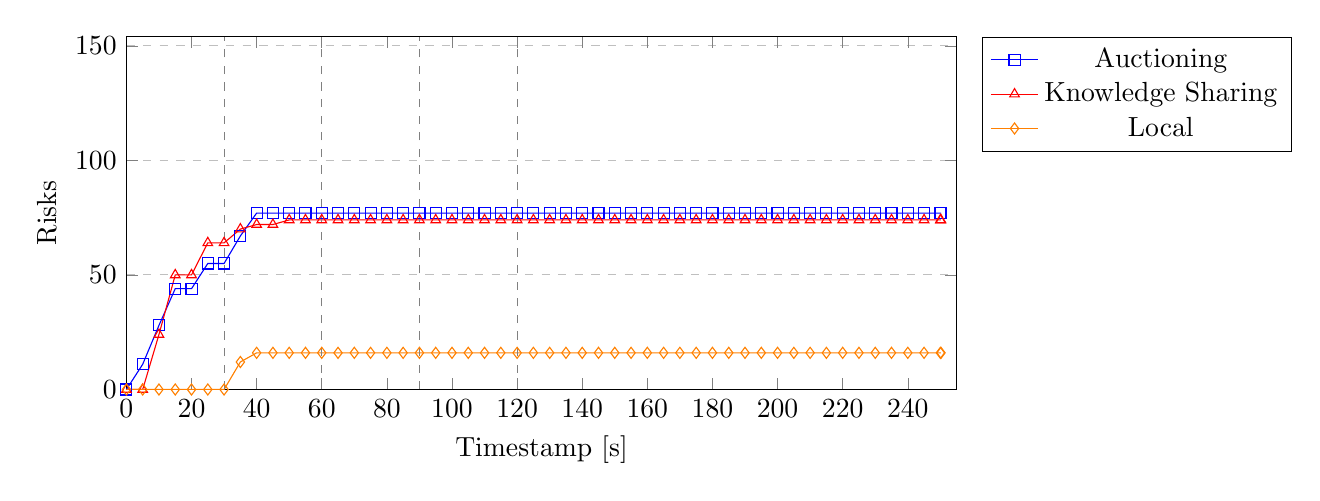
\begin{tikzpicture}
\begin{axis}[
    xlabel={Timestamp [s]},
    ylabel={Risks},
    xmin=0, xmax=255000,
    ymin=0, ymax=154,
    legend pos=outer north east,
    ymajorgrids=true,
    grid style=dashed,
    width=\textwidth,
    height=0.5\textwidth,
    scaled x ticks=base 10:-3,
    xtick scale label code/.code={}
]

	\addplot[color=blue,mark=square] coordinates {
        (0,0)(5000,11)(10000,28)(15000,44)(20000,44)(25000,55)(30000,55)(35000,67)(40000,77)(45000,77)(50000,77)(55000,77)(60000,77)(65000,77)(70000,77)(75000,77)(80000,77)(85000,77)(90000,77)(95000,77)(100000,77)(105000,77)(110000,77)(115000,77)(120000,77)(125000,77)(130000,77)(135000,77)(140000,77)(145000,77)(150000,77)(155000,77)(160000,77)(165000,77)(170000,77)(175000,77)(180000,77)(185000,77)(190000,77)(195000,77)(200000,77)(205000,77)(210000,77)(215000,77)(220000,77)(225000,77)(230000,77)(235000,77)(240000,77)(245000,77)(250000,77)(250270,77)
    };
    \addlegendentry{Auctioning}
	\addplot[color=red,mark=triangle] coordinates {
        (0,0)(5000,0)(10000,24)(15000,50)(20000,50)(25000,64)(30000,64)(35000,70)(40000,72)(45000,72)(50000,74)(55000,74)(60000,74)(65000,74)(70000,74)(75000,74)(80000,74)(85000,74)(90000,74)(95000,74)(100000,74)(105000,74)(110000,74)(115000,74)(120000,74)(125000,74)(130000,74)(135000,74)(140000,74)(145000,74)(150000,74)(155000,74)(160000,74)(165000,74)(170000,74)(175000,74)(180000,74)(185000,74)(190000,74)(195000,74)(200000,74)(205000,74)(210000,74)(215000,74)(220000,74)(225000,74)(230000,74)(235000,74)(240000,74)(245000,74)(250000,74)(250172,74)
    };
    \addlegendentry{Knowledge Sharing}
	\addplot[color=orange,mark=diamond] coordinates {
        (0,0)(5000,0)(10000,0)(15000,0)(20000,0)(25000,0)(30000,0)(35000,12)(40000,16)(45000,16)(50000,16)(55000,16)(60000,16)(65000,16)(70000,16)(75000,16)(80000,16)(85000,16)(90000,16)(95000,16)(100000,16)(105000,16)(110000,16)(115000,16)(120000,16)(125000,16)(130000,16)(135000,16)(140000,16)(145000,16)(150000,16)(155000,16)(160000,16)(165000,16)(170000,16)(175000,16)(180000,16)(185000,16)(190000,16)(195000,16)(200000,16)(205000,16)(210000,16)(215000,16)(220000,16)(225000,16)(230000,16)(235000,16)(240000,16)(245000,16)(250000,16)(250190,16)
    };
    \addlegendentry{Local}

	\addplot[color=gray, dashed,] coordinates {(30000,0) (30000,154)};
	\addplot[color=gray, dashed,] coordinates {(60000,0) (60000,154)};
	\addplot[color=gray, dashed,] coordinates {(90000,0) (90000,154)};
	\addplot[color=gray, dashed,] coordinates {(120000,0) (120000,154)};


\end{axis}
\end{tikzpicture}
    \caption{Graph showing the number of unique risks detected by agents in the unstable scenario.}
    \label{fig:risk-count-unstable}
\end{figure}

\begin{figure}[H]
    \centering
        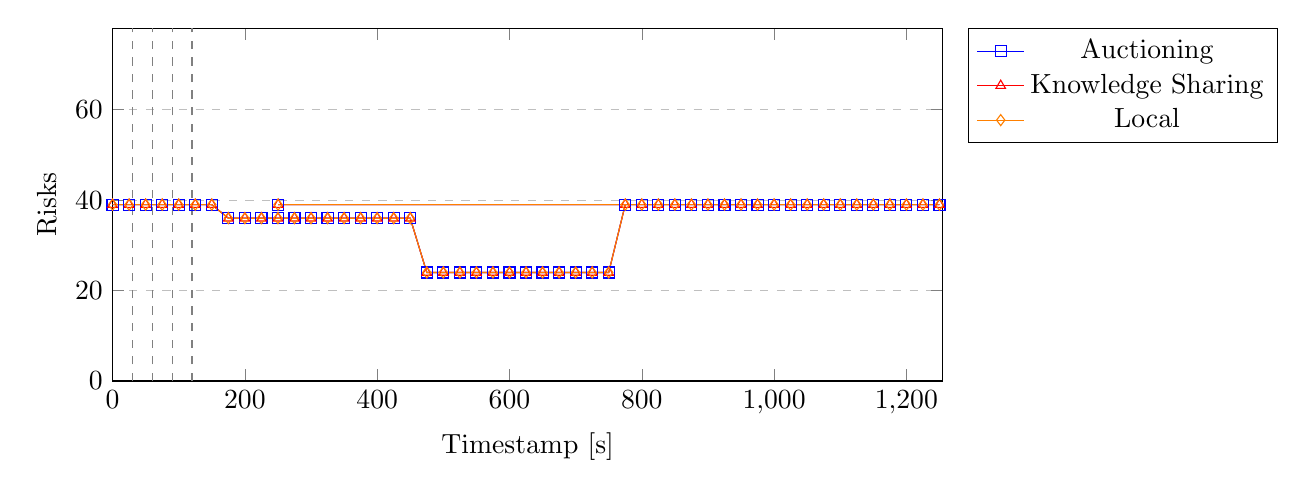
\begin{tikzpicture}
\begin{axis}[
    xlabel={Timestamp [s]},
    ylabel={Risks},
    xmin=0, xmax=1255000,
    ymin=0, ymax=78,
    legend pos=outer north east,
    ymajorgrids=true,
    grid style=dashed,
    width=\textwidth,
    height=0.5\textwidth,
    scaled x ticks=base 10:-3,
    xtick scale label code/.code={}
]

	\addplot[color=blue,mark=square] coordinates {
        (0,39)(25000,39)(50000,39)(75000,39)(100000,39)(125000,39)(150000,39)(175000,36)(200000,36)(225000,36)(250000,36)(275000,36)(300000,36)(325000,36)(350000,36)(375000,36)(400000,36)(425000,36)(450000,36)(475000,24)(500000,24)(525000,24)(550000,24)(575000,24)(600000,24)(625000,24)(650000,24)(675000,24)(700000,24)(725000,24)(750000,24)(775000,39)(800000,39)(825000,39)(850000,39)(875000,39)(900000,39)(925000,39)(950000,39)(975000,39)(1000000,39)(1025000,39)(1050000,39)(1075000,39)(1100000,39)(1125000,39)(1150000,39)(1175000,39)(1200000,39)(1225000,39)(1250000,39)(250362,39)
    };
    \addlegendentry{Auctioning}
	\addplot[color=red,mark=triangle] coordinates {
        (0,39)(25000,39)(50000,39)(75000,39)(100000,39)(125000,39)(150000,39)(175000,36)(200000,36)(225000,36)(250000,36)(275000,36)(300000,36)(325000,36)(350000,36)(375000,36)(400000,36)(425000,36)(450000,36)(475000,24)(500000,24)(525000,24)(550000,24)(575000,24)(600000,24)(625000,24)(650000,24)(675000,24)(700000,24)(725000,24)(750000,24)(775000,39)(800000,39)(825000,39)(850000,39)(875000,39)(900000,39)(925000,39)(950000,39)(975000,39)(1000000,39)(1025000,39)(1050000,39)(1075000,39)(1100000,39)(1125000,39)(1150000,39)(1175000,39)(1200000,39)(1225000,39)(1250000,39)(250334,39)
    };
    \addlegendentry{Knowledge Sharing}
	\addplot[color=orange,mark=diamond] coordinates {
        (0,39)(25000,39)(50000,39)(75000,39)(100000,39)(125000,39)(150000,39)(175000,36)(200000,36)(225000,36)(250000,36)(275000,36)(300000,36)(325000,36)(350000,36)(375000,36)(400000,36)(425000,36)(450000,36)(475000,24)(500000,24)(525000,24)(550000,24)(575000,24)(600000,24)(625000,24)(650000,24)(675000,24)(700000,24)(725000,24)(750000,24)(775000,39)(800000,39)(825000,39)(850000,39)(875000,39)(900000,39)(925000,39)(950000,39)(975000,39)(1000000,39)(1025000,39)(1050000,39)(1075000,39)(1100000,39)(1125000,39)(1150000,39)(1175000,39)(1200000,39)(1225000,39)(1250000,39)(250168,39)
    };
    \addlegendentry{Local}

	\addplot[color=gray, dashed,] coordinates {(30000,0) (30000,78)};
	\addplot[color=gray, dashed,] coordinates {(60000,0) (60000,78)};
	\addplot[color=gray, dashed,] coordinates {(90000,0) (90000,78)};
	\addplot[color=gray, dashed,] coordinates {(120000,0) (120000,78)};


\end{axis}
\end{tikzpicture}
    \caption{Graph showing the number of remaining risks in the infrastructure in the unstable scenario.}
    \label{fig:risk-remaining-unstable}
\end{figure}

\add{write}

\begin{figure}[H]
    \hspace*{-1cm}
    \centering
        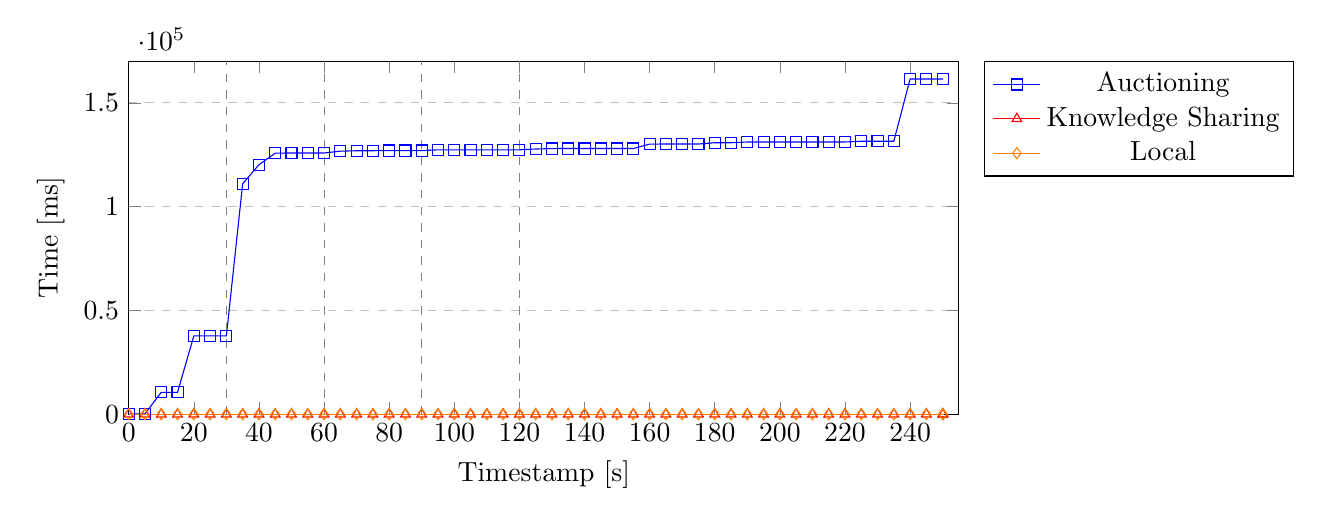
\begin{tikzpicture}
\begin{axis}[
    xlabel={Timestamp [s]},
    ylabel={Time [ms]},
    xmin=0, xmax=255000,
    ymin=0, ymax=170017,
    legend pos=outer north east,
    ymajorgrids=true,
    grid style=dashed,
    width=\textwidth,
    height=0.5\textwidth,
    scaled x ticks=base 10:-3,
    xtick scale label code/.code={}
]

	\addplot[color=blue,mark=square] coordinates {
        (0,0)(5000,173)(10000,10538)(15000,10538)(20000,37730)(25000,37730)(30000,37730)(35000,111030)(40000,120177)(45000,125786)(50000,125855)(55000,125855)(60000,125855)(65000,126731)(70000,126932)(75000,126952)(80000,127013)(85000,127013)(90000,127013)(95000,127365)(100000,127365)(105000,127385)(110000,127385)(115000,127385)(120000,127385)(125000,127764)(130000,127985)(135000,128006)(140000,128006)(145000,128006)(150000,128006)(155000,128006)(160000,130144)(165000,130172)(170000,130172)(175000,130172)(180000,130795)(185000,130795)(190000,131135)(195000,131135)(200000,131161)(205000,131161)(210000,131161)(215000,131161)(220000,131161)(225000,131489)(230000,131517)(235000,131517)(240000,161517)(245000,161517)(250000,161517)(250144,161517)
    };
    \addlegendentry{Auctioning}
	\addplot[color=red,mark=triangle] coordinates {
        (0,0)(5000,0)(10000,0)(15000,0)(20000,0)(25000,0)(30000,0)(35000,0)(40000,0)(45000,0)(50000,0)(55000,0)(60000,0)(65000,0)(70000,0)(75000,0)(80000,0)(85000,0)(90000,0)(95000,0)(100000,0)(105000,0)(110000,0)(115000,0)(120000,0)(125000,0)(130000,0)(135000,0)(140000,0)(145000,0)(150000,0)(155000,0)(160000,0)(165000,0)(170000,0)(175000,0)(180000,0)(185000,0)(190000,0)(195000,0)(200000,0)(205000,0)(210000,0)(215000,0)(220000,0)(225000,0)(230000,0)(235000,0)(240000,0)(245000,0)(250000,0)(250118,0)
    };
    \addlegendentry{Knowledge Sharing}
	\addplot[color=orange,mark=diamond] coordinates {
        (0,0)(5000,0)(10000,0)(15000,0)(20000,0)(25000,0)(30000,0)(35000,0)(40000,0)(45000,0)(50000,0)(55000,0)(60000,0)(65000,0)(70000,0)(75000,0)(80000,0)(85000,0)(90000,0)(95000,0)(100000,0)(105000,0)(110000,0)(115000,0)(120000,0)(125000,0)(130000,0)(135000,0)(140000,0)(145000,0)(150000,0)(155000,0)(160000,0)(165000,0)(170000,0)(175000,0)(180000,0)(185000,0)(190000,0)(195000,0)(200000,0)(205000,0)(210000,0)(215000,0)(220000,0)(225000,0)(230000,0)(235000,0)(240000,0)(245000,0)(250000,0)(250091,0)
    };
    \addlegendentry{Local}

	\addplot[color=gray, dashed,] coordinates {(30000,0) (30000,170017)};
	\addplot[color=gray, dashed,] coordinates {(60000,0) (60000,170017)};
	\addplot[color=gray, dashed,] coordinates {(90000,0) (90000,170017)};
	\addplot[color=gray, dashed,] coordinates {(120000,0) (120000,170017)};


\end{axis}
\end{tikzpicture}
    \caption{Graph showing the sum of time spent auctioning by agents in the unstable scenario.}
    \label{fig:auctioning-time-unstable}
\end{figure}

\begin{figure}[H]
    \hspace*{-1cm}
    \centering
        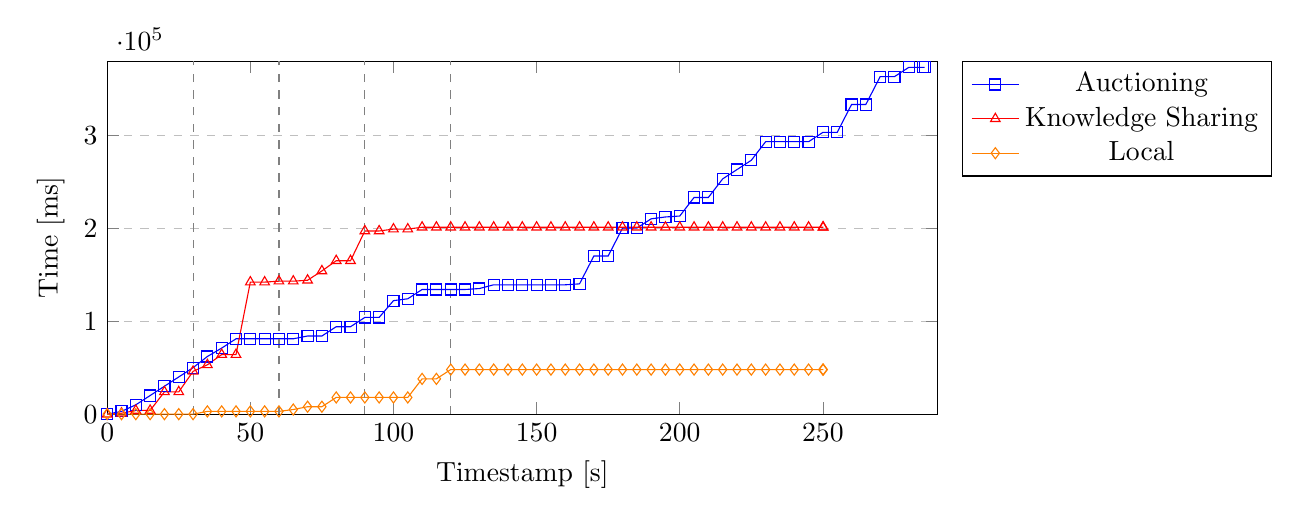
\begin{tikzpicture}
\begin{axis}[
    xlabel={Timestamp [s]},
    ylabel={Time [ms]},
    xmin=0, xmax=290000,
    ymin=0, ymax=380038,
    legend pos=outer north east,
    ymajorgrids=true,
    grid style=dashed,
    width=\textwidth,
    height=0.5\textwidth,
    scaled x ticks=base 10:-3,
    xtick scale label code/.code={}
]

	\addplot[color=blue,mark=square] coordinates {
        (0,0)(5000,3015)(10000,10073)(15000,20083)(20000,30092)(25000,40100)(30000,50105)(35000,62134)(40000,71193)(45000,81199)(50000,81199)(55000,81199)(60000,81199)(65000,81199)(70000,84209)(75000,84209)(80000,94219)(85000,94219)(90000,104222)(95000,104222)(100000,122281)(105000,124295)(110000,134306)(115000,134306)(120000,134306)(125000,134306)(130000,135314)(135000,139351)(140000,139351)(145000,139351)(150000,139351)(155000,139351)(160000,139351)(165000,140360)(170000,170377)(175000,170377)(180000,200396)(185000,200396)(190000,210405)(195000,212415)(200000,213423)(205000,233437)(210000,233437)(215000,253455)(220000,263466)(225000,273475)(230000,293490)(235000,293490)(240000,293490)(245000,293490)(250000,303496)(255000,303496)(260000,333521)(265000,333521)(270000,363542)(275000,363542)(280000,373547)(285000,373547)(285530,373547)
    };
    \addlegendentry{Auctioning}
	\addplot[color=red,mark=triangle] coordinates {
        (0,0)(5000,1009)(10000,4030)(15000,4030)(20000,24044)(25000,24044)(30000,46078)(35000,53188)(40000,64205)(45000,64205)(50000,142255)(55000,142255)(60000,143258)(65000,143258)(70000,144266)(75000,154274)(80000,165289)(85000,165289)(90000,197316)(95000,197316)(100000,199335)(105000,199335)(110000,201346)(115000,201346)(120000,201346)(125000,201346)(130000,201346)(135000,201346)(140000,201346)(145000,201346)(150000,201346)(155000,201346)(160000,201346)(165000,201346)(170000,201346)(175000,201346)(180000,201346)(185000,201346)(190000,201346)(195000,201346)(200000,201346)(205000,201346)(210000,201346)(215000,201346)(220000,201346)(225000,201346)(230000,201346)(235000,201346)(240000,201346)(245000,201346)(250000,201346)(250138,201346)
    };
    \addlegendentry{Knowledge Sharing}
	\addplot[color=orange,mark=diamond] coordinates {
        (0,0)(5000,0)(10000,0)(15000,0)(20000,0)(25000,0)(30000,0)(35000,3011)(40000,3011)(45000,3011)(50000,3011)(55000,3011)(60000,3011)(65000,5019)(70000,8033)(75000,8033)(80000,18038)(85000,18038)(90000,18038)(95000,18038)(100000,18038)(105000,18038)(110000,38043)(115000,38043)(120000,48045)(125000,48045)(130000,48045)(135000,48045)(140000,48045)(145000,48045)(150000,48045)(155000,48045)(160000,48045)(165000,48045)(170000,48045)(175000,48045)(180000,48045)(185000,48045)(190000,48045)(195000,48045)(200000,48045)(205000,48045)(210000,48045)(215000,48045)(220000,48045)(225000,48045)(230000,48045)(235000,48045)(240000,48045)(245000,48045)(250000,48045)(250134,48045)
    };
    \addlegendentry{Local}

	\addplot[color=gray, dashed,] coordinates {(30000,0) (30000,380038)};
	\addplot[color=gray, dashed,] coordinates {(60000,0) (60000,380038)};
	\addplot[color=gray, dashed,] coordinates {(90000,0) (90000,380038)};
	\addplot[color=gray, dashed,] coordinates {(120000,0) (120000,380038)};


\end{axis}
\end{tikzpicture}
    \caption{Graph showing the sum of time spent adapting by agents in the unstable scenario.}
    \label{fig:adapting-time-unstable}
\end{figure}

As with the prior graphs for this scenario we see that Figure \ref{fig:adapting-time-unstable} is also stable after the first $50$ seconds. There are no new risks as shown in Figure \ref{fig:risk-count-unstable} and no new adaptations are necessary to mitigate them. 



\subsection*{Consecutive runs}
\begin{figure}[H]
    \centering
        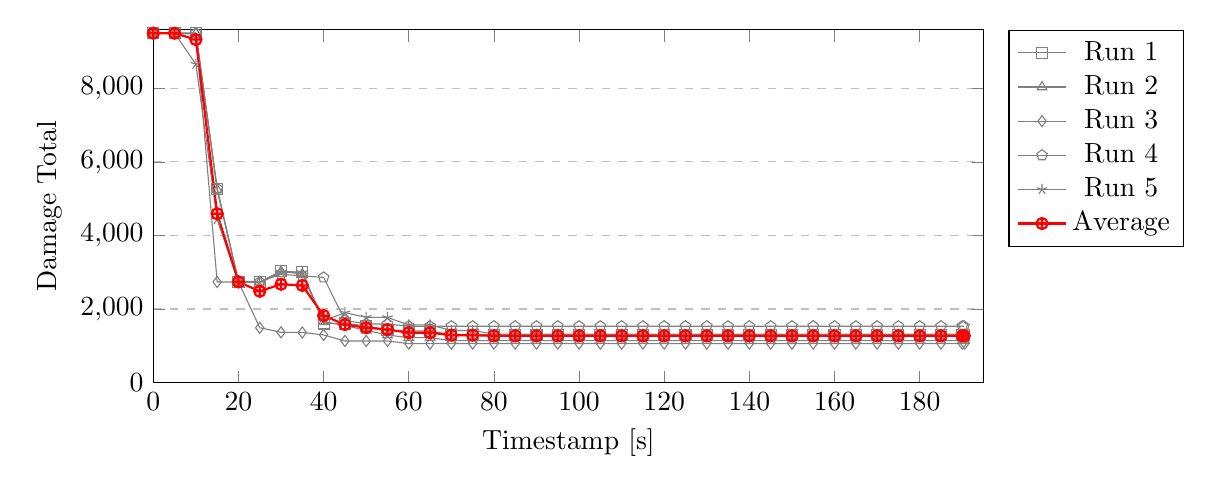
\begin{tikzpicture}
\begin{axis}[
    xlabel={Timestamp [s]},
    ylabel={Damage Total},
    xmin=0, xmax=195000,
    ymin=0, ymax=9595,
    legend pos=outer north east,
    ymajorgrids=true,
    grid style=dashed,
    width=\textwidth,
    height=0.5\textwidth,
    scaled x ticks=base 10:-3,
    xtick scale label code/.code={}
]

	\addplot[color=gray,mark=square] coordinates {
        (0,9500.86)(5000,9500.86)(10000,9500.86)(15000,5273.46)(20000,2735.67)(25000,2733.78)(30000,3030.23)(35000,2999.27)(40000,1606.26)(45000,1606.26)(50000,1545.84)(55000,1424.29)(60000,1401.35)(65000,1401.35)(70000,1299.55)(75000,1299.55)(80000,1299.55)(85000,1299.55)(90000,1299.55)(95000,1299.55)(100000,1299.55)(105000,1299.55)(110000,1299.55)(115000,1299.55)(120000,1299.55)(125000,1299.55)(130000,1299.55)(135000,1299.55)(140000,1299.55)(145000,1299.55)(150000,1299.55)(155000,1299.55)(160000,1299.55)(165000,1299.55)(170000,1299.55)(175000,1299.55)(180000,1299.55)(185000,1299.55)(190000,1299.55)(190469,1299.55)
    };
    \addlegendentry{Run 1}
	\addplot[color=gray,mark=triangle] coordinates {
        (0,9500.86)(5000,9500.86)(10000,9500.86)(15000,5244.51)(20000,2735.67)(25000,2733.78)(30000,3027.26)(35000,2951.72)(40000,1657.47)(45000,1550.25)(50000,1420.21)(55000,1293.76)(60000,1220.39)(65000,1220.39)(70000,1142.59)(75000,1142.59)(80000,1142.59)(85000,1142.59)(90000,1142.59)(95000,1142.59)(100000,1142.59)(105000,1142.59)(110000,1142.59)(115000,1142.59)(120000,1142.59)(125000,1142.59)(130000,1142.59)(135000,1142.59)(140000,1142.59)(145000,1142.59)(150000,1142.59)(155000,1142.59)(160000,1142.59)(165000,1142.59)(170000,1142.59)(175000,1142.59)(180000,1142.59)(185000,1142.59)(190000,1142.59)(190603,1142.59)
    };
    \addlegendentry{Run 2}
	\addplot[color=gray,mark=diamond] coordinates {
        (0,9500.86)(5000,9500.86)(10000,9475.27)(15000,2735.67)(20000,2735.67)(25000,1491.74)(30000,1368.06)(35000,1362.13)(40000,1296.28)(45000,1131.00)(50000,1131.00)(55000,1131.00)(60000,1059.17)(65000,1059.17)(70000,1059.17)(75000,1059.17)(80000,1059.17)(85000,1059.17)(90000,1059.17)(95000,1059.17)(100000,1059.17)(105000,1059.17)(110000,1059.17)(115000,1059.17)(120000,1059.17)(125000,1059.17)(130000,1059.17)(135000,1059.17)(140000,1059.17)(145000,1059.17)(150000,1059.17)(155000,1059.17)(160000,1059.17)(165000,1059.17)(170000,1059.17)(175000,1059.17)(180000,1059.17)(185000,1059.17)(190000,1059.17)(190583,1059.17)
    };
    \addlegendentry{Run 3}
	\addplot[color=gray,mark=pentagon] coordinates {
        (0,9500.86)(5000,9500.86)(10000,9500.86)(15000,5273.46)(20000,2757.80)(25000,2735.67)(30000,2946.76)(35000,2901.60)(40000,2859.47)(45000,1695.56)(50000,1592.95)(55000,1592.95)(60000,1531.57)(65000,1531.57)(70000,1531.57)(75000,1531.57)(80000,1531.57)(85000,1531.57)(90000,1531.57)(95000,1531.57)(100000,1531.57)(105000,1531.57)(110000,1531.57)(115000,1531.57)(120000,1531.57)(125000,1531.57)(130000,1531.57)(135000,1531.57)(140000,1531.57)(145000,1531.57)(150000,1531.57)(155000,1531.57)(160000,1531.57)(165000,1531.57)(170000,1531.57)(175000,1531.57)(180000,1531.57)(185000,1531.57)(190000,1531.57)(190405,1531.57)
    };
    \addlegendentry{Run 4}
	\addplot[color=gray,mark=star] coordinates {
        (0,9500.86)(5000,9500.86)(10000,8658.83)(15000,4434.90)(20000,2726.22)(25000,2726.22)(30000,3000.82)(35000,2997.05)(40000,1685.04)(45000,1899.99)(50000,1777.19)(55000,1769.17)(60000,1569.23)(65000,1569.23)(70000,1417.12)(75000,1417.12)(80000,1318.25)(85000,1318.25)(90000,1318.25)(95000,1318.25)(100000,1318.25)(105000,1318.25)(110000,1318.25)(115000,1318.25)(120000,1318.25)(125000,1318.25)(130000,1318.25)(135000,1318.25)(140000,1318.25)(145000,1318.25)(150000,1318.25)(155000,1318.25)(160000,1318.25)(165000,1318.25)(170000,1318.25)(175000,1318.25)(180000,1318.25)(185000,1318.25)(190000,1318.25)(190567,1318.25)
    };
    \addlegendentry{Run 5}
	\addplot[color=red,mark=oplus,thick] coordinates {
        (0,9500)(5000,9500)(10000,9326.6)(15000,4591.8)(20000,2737.6)(25000,2483.6)(30000,2674.2)(35000,2642)(40000,1820.6)(45000,1576.2)(50000,1493)(55000,1441.8)(60000,1356)(65000,1356)(70000,1289.6)(75000,1289.6)(80000,1269.8)(85000,1269.8)(90000,1269.8)(95000,1269.8)(100000,1269.8)(105000,1269.8)(110000,1269.8)(115000,1269.8)(120000,1269.8)(125000,1269.8)(130000,1269.8)(135000,1269.8)(140000,1269.8)(145000,1269.8)(150000,1269.8)(155000,1269.8)(160000,1269.8)(165000,1269.8)(170000,1269.8)(175000,1269.8)(180000,1269.8)(185000,1269.8)(190000,1269.8)(190469,1269.8)
    };
    \addlegendentry{Average}
\end{axis}
\end{tikzpicture}

    \caption{Graph showing the Auctioning Feature's performance over multiple runs in the no-change scenario.}
\end{figure}

\subsection*{Small Infrastructure}
\begin{figure}[H]
    \centering
        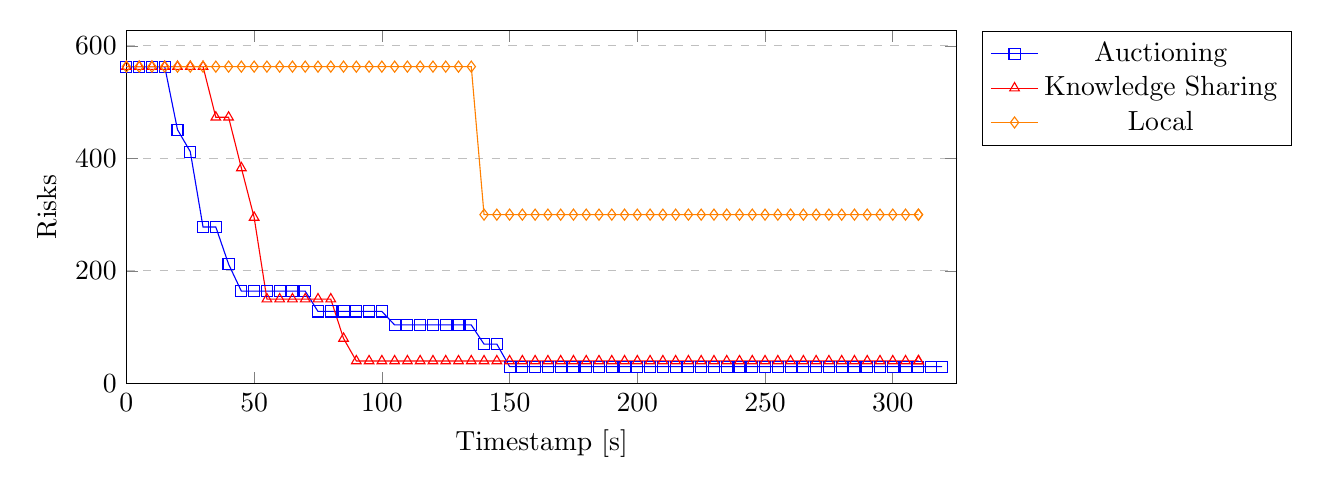
\begin{tikzpicture}
\begin{axis}[
    xlabel={Timestamp [s]},
    ylabel={Risks},
    xmin=0, xmax=325000,
    ymin=0, ymax=627,
    legend pos=outer north east,
    ymajorgrids=true,
    grid style=dashed,
    width=\textwidth,
    height=0.5\textwidth,
    scaled x ticks=base 10:-3,
    xtick scale label code/.code={}
]

	\addplot[color=blue,mark=square] coordinates {
        (0,563)(5000,563)(10000,563)(15000,563)(20000,451)(25000,412)(30000,278)(35000,278)(40000,212)(45000,164)(50000,164)(55000,164)(60000,164)(65000,164)(70000,164)(75000,128)(80000,128)(85000,128)(90000,128)(95000,128)(100000,128)(105000,104)(110000,104)(115000,104)(120000,104)(125000,104)(130000,104)(135000,104)(140000,70)(145000,70)(150000,30)(155000,30)(160000,30)(165000,30)(170000,30)(175000,30)(180000,30)(185000,30)(190000,30)(195000,30)(200000,30)(205000,30)(210000,30)(215000,30)(220000,30)(225000,30)(230000,30)(235000,30)(240000,30)(245000,30)(250000,30)(255000,30)(260000,30)(265000,30)(270000,30)(275000,30)(280000,30)(285000,30)(290000,30)(295000,30)(300000,30)(305000,30)(310000,30)(315000,30)(319272,30)
    };
    \addlegendentry{Auctioning}
	\addplot[color=red,mark=triangle] coordinates {
        (0,563)(5000,563)(10000,563)(15000,563)(20000,563)(25000,563)(30000,563)(35000,473)(40000,473)(45000,383)(50000,295)(55000,150)(60000,150)(65000,150)(70000,150)(75000,150)(80000,150)(85000,80)(90000,40)(95000,40)(100000,40)(105000,40)(110000,40)(115000,40)(120000,40)(125000,40)(130000,40)(135000,40)(140000,40)(145000,40)(150000,40)(155000,40)(160000,40)(165000,40)(170000,40)(175000,40)(180000,40)(185000,40)(190000,40)(195000,40)(200000,40)(205000,40)(210000,40)(215000,40)(220000,40)(225000,40)(230000,40)(235000,40)(240000,40)(245000,40)(250000,40)(255000,40)(260000,40)(265000,40)(270000,40)(275000,40)(280000,40)(285000,40)(290000,40)(295000,40)(300000,40)(305000,40)(310000,40)(310115,40)
    };
    \addlegendentry{Knowledge Sharing}
	\addplot[color=orange,mark=diamond] coordinates {
        (0,563)(5000,563)(10000,563)(15000,563)(20000,563)(25000,563)(30000,563)(35000,563)(40000,563)(45000,563)(50000,563)(55000,563)(60000,563)(65000,563)(70000,563)(75000,563)(80000,563)(85000,563)(90000,563)(95000,563)(100000,563)(105000,563)(110000,563)(115000,563)(120000,563)(125000,563)(130000,563)(135000,563)(140000,300)(145000,300)(150000,300)(155000,300)(160000,300)(165000,300)(170000,300)(175000,300)(180000,300)(185000,300)(190000,300)(195000,300)(200000,300)(205000,300)(210000,300)(215000,300)(220000,300)(225000,300)(230000,300)(235000,300)(240000,300)(245000,300)(250000,300)(255000,300)(260000,300)(265000,300)(270000,300)(275000,300)(280000,300)(285000,300)(290000,300)(295000,300)(300000,300)(305000,300)(310000,300)(310098,300)
    };
    \addlegendentry{Local}




\end{axis}
\end{tikzpicture}
    \caption{Graph showing the output of all feature sets in the non-changing scenario, with a small infrastructure.}
\end{figure}
